% Options for packages loaded elsewhere
\PassOptionsToPackage{unicode}{hyperref}
\PassOptionsToPackage{hyphens}{url}
%
\documentclass[
]{article}
\usepackage{amsmath,amssymb}
\usepackage{iftex}
\ifPDFTeX
  \usepackage[T1]{fontenc}
  \usepackage[utf8]{inputenc}
  \usepackage{textcomp} % provide euro and other symbols
\else % if luatex or xetex
  \usepackage{unicode-math} % this also loads fontspec
  \defaultfontfeatures{Scale=MatchLowercase}
  \defaultfontfeatures[\rmfamily]{Ligatures=TeX,Scale=1}
\fi
\usepackage{lmodern}
\ifPDFTeX\else
  % xetex/luatex font selection
\fi
% Use upquote if available, for straight quotes in verbatim environments
\IfFileExists{upquote.sty}{\usepackage{upquote}}{}
\IfFileExists{microtype.sty}{% use microtype if available
  \usepackage[]{microtype}
  \UseMicrotypeSet[protrusion]{basicmath} % disable protrusion for tt fonts
}{}
\makeatletter
\@ifundefined{KOMAClassName}{% if non-KOMA class
  \IfFileExists{parskip.sty}{%
    \usepackage{parskip}
  }{% else
    \setlength{\parindent}{0pt}
    \setlength{\parskip}{6pt plus 2pt minus 1pt}}
}{% if KOMA class
  \KOMAoptions{parskip=half}}
\makeatother
\usepackage{xcolor}
\usepackage[margin=1in]{geometry}
\usepackage{color}
\usepackage{fancyvrb}
\newcommand{\VerbBar}{|}
\newcommand{\VERB}{\Verb[commandchars=\\\{\}]}
\DefineVerbatimEnvironment{Highlighting}{Verbatim}{commandchars=\\\{\}}
% Add ',fontsize=\small' for more characters per line
\usepackage{framed}
\definecolor{shadecolor}{RGB}{248,248,248}
\newenvironment{Shaded}{\begin{snugshade}}{\end{snugshade}}
\newcommand{\AlertTok}[1]{\textcolor[rgb]{0.94,0.16,0.16}{#1}}
\newcommand{\AnnotationTok}[1]{\textcolor[rgb]{0.56,0.35,0.01}{\textbf{\textit{#1}}}}
\newcommand{\AttributeTok}[1]{\textcolor[rgb]{0.13,0.29,0.53}{#1}}
\newcommand{\BaseNTok}[1]{\textcolor[rgb]{0.00,0.00,0.81}{#1}}
\newcommand{\BuiltInTok}[1]{#1}
\newcommand{\CharTok}[1]{\textcolor[rgb]{0.31,0.60,0.02}{#1}}
\newcommand{\CommentTok}[1]{\textcolor[rgb]{0.56,0.35,0.01}{\textit{#1}}}
\newcommand{\CommentVarTok}[1]{\textcolor[rgb]{0.56,0.35,0.01}{\textbf{\textit{#1}}}}
\newcommand{\ConstantTok}[1]{\textcolor[rgb]{0.56,0.35,0.01}{#1}}
\newcommand{\ControlFlowTok}[1]{\textcolor[rgb]{0.13,0.29,0.53}{\textbf{#1}}}
\newcommand{\DataTypeTok}[1]{\textcolor[rgb]{0.13,0.29,0.53}{#1}}
\newcommand{\DecValTok}[1]{\textcolor[rgb]{0.00,0.00,0.81}{#1}}
\newcommand{\DocumentationTok}[1]{\textcolor[rgb]{0.56,0.35,0.01}{\textbf{\textit{#1}}}}
\newcommand{\ErrorTok}[1]{\textcolor[rgb]{0.64,0.00,0.00}{\textbf{#1}}}
\newcommand{\ExtensionTok}[1]{#1}
\newcommand{\FloatTok}[1]{\textcolor[rgb]{0.00,0.00,0.81}{#1}}
\newcommand{\FunctionTok}[1]{\textcolor[rgb]{0.13,0.29,0.53}{\textbf{#1}}}
\newcommand{\ImportTok}[1]{#1}
\newcommand{\InformationTok}[1]{\textcolor[rgb]{0.56,0.35,0.01}{\textbf{\textit{#1}}}}
\newcommand{\KeywordTok}[1]{\textcolor[rgb]{0.13,0.29,0.53}{\textbf{#1}}}
\newcommand{\NormalTok}[1]{#1}
\newcommand{\OperatorTok}[1]{\textcolor[rgb]{0.81,0.36,0.00}{\textbf{#1}}}
\newcommand{\OtherTok}[1]{\textcolor[rgb]{0.56,0.35,0.01}{#1}}
\newcommand{\PreprocessorTok}[1]{\textcolor[rgb]{0.56,0.35,0.01}{\textit{#1}}}
\newcommand{\RegionMarkerTok}[1]{#1}
\newcommand{\SpecialCharTok}[1]{\textcolor[rgb]{0.81,0.36,0.00}{\textbf{#1}}}
\newcommand{\SpecialStringTok}[1]{\textcolor[rgb]{0.31,0.60,0.02}{#1}}
\newcommand{\StringTok}[1]{\textcolor[rgb]{0.31,0.60,0.02}{#1}}
\newcommand{\VariableTok}[1]{\textcolor[rgb]{0.00,0.00,0.00}{#1}}
\newcommand{\VerbatimStringTok}[1]{\textcolor[rgb]{0.31,0.60,0.02}{#1}}
\newcommand{\WarningTok}[1]{\textcolor[rgb]{0.56,0.35,0.01}{\textbf{\textit{#1}}}}
\usepackage{graphicx}
\makeatletter
\newsavebox\pandoc@box
\newcommand*\pandocbounded[1]{% scales image to fit in text height/width
  \sbox\pandoc@box{#1}%
  \Gscale@div\@tempa{\textheight}{\dimexpr\ht\pandoc@box+\dp\pandoc@box\relax}%
  \Gscale@div\@tempb{\linewidth}{\wd\pandoc@box}%
  \ifdim\@tempb\p@<\@tempa\p@\let\@tempa\@tempb\fi% select the smaller of both
  \ifdim\@tempa\p@<\p@\scalebox{\@tempa}{\usebox\pandoc@box}%
  \else\usebox{\pandoc@box}%
  \fi%
}
% Set default figure placement to htbp
\def\fps@figure{htbp}
\makeatother
\setlength{\emergencystretch}{3em} % prevent overfull lines
\providecommand{\tightlist}{%
  \setlength{\itemsep}{0pt}\setlength{\parskip}{0pt}}
\setcounter{secnumdepth}{5}
\usepackage{bookmark}
\IfFileExists{xurl.sty}{\usepackage{xurl}}{} % add URL line breaks if available
\urlstyle{same}
\hypersetup{
  pdftitle={Das Berufsbild des Data Scienctisten aufgeschlüsselt},
  hidelinks,
  pdfcreator={LaTeX via pandoc}}

\title{Das Berufsbild des Data Scienctisten aufgeschlüsselt}
\author{}
\date{\vspace{-2.5em}}

\begin{document}
\maketitle

{
\setcounter{tocdepth}{3}
\tableofcontents
}
\section{Einleitung}\label{einleitung}

\subsection{Requirements}\label{requirements}

Zunächst müssen die benötigten Bibliotheken installiert werden:

\begin{Shaded}
\begin{Highlighting}[]
\CommentTok{\#install.packages("tidyverse")}
\CommentTok{\#install.packages("igraph")}
\CommentTok{\#install.packages("visNetwork")}
\CommentTok{\#install.packages("dplyr")}
\CommentTok{\#install.packages("tidyr")}
\end{Highlighting}
\end{Shaded}

\begin{Shaded}
\begin{Highlighting}[]
\CommentTok{\# Bibliotheken laden}
\FunctionTok{library}\NormalTok{(tidyverse)}
\FunctionTok{library}\NormalTok{(igraph)}
\FunctionTok{library}\NormalTok{(visNetwork)}
\FunctionTok{library}\NormalTok{(dplyr)}
\FunctionTok{library}\NormalTok{(tidyr)}
\end{Highlighting}
\end{Shaded}

\subsection{Motivation und
Zielsetzung}\label{motivation-und-zielsetzung}

In ihrem Artikel ``Data Scientist: The Sexiest Job of the 21st Century''
betonen Davenport und Patil, dass Data Scientists durch ihre Fähigkeiten
in Informatik, Statistik und ihr Fachwissen allgemein einen erheblichen
Mehrwert für Unternehmen schaffen.\footnote{Davenport, Patil 2012} Die
Fähigkeit, aus komplexen, unstrukturierten Daten wertvolle Erkenntnisse
zu gewinnen, macht Data Scientists in vielen Branchen zu einer
unverzichtbaren Ressource.\footnote{Davenport, Patil 2012} Die Nutzung
ihrer Kompetenzen verschafft Unternehmen einen Wettbewerbsvorteil, da
sie datengetriebene Entscheidungen, Produktinnovationen und
Effizienzsteigerungen ermöglicht.\footnote{Davenport, Patil 2012}

Darüber ob Data Scientists immer noch the ``Sexiest Job'' des 21.
Jahrhunderts sind, lässt sich streiten. Fakt ist jedoch, dass die
Nachfrage nach Data Scientists in den letzten Jahren stark gestiegen ist
und vorraussichtlich immer weiter steigen wird. Dieser Trend ist auch in
den Google-Suchanfragen zu den Begriffen erkenntlich:\footnote{Google
  Trends, abgerufen am 30.10.2024}

\begin{Shaded}
\begin{Highlighting}[]
\FunctionTok{ggplot}\NormalTok{(data, }\FunctionTok{aes}\NormalTok{(}\AttributeTok{x =}\NormalTok{ Monat)) }\SpecialCharTok{+}
  \FunctionTok{geom\_line}\NormalTok{(}\FunctionTok{aes}\NormalTok{(}\AttributeTok{y =} \StringTok{\textasciigrave{}}\AttributeTok{data science}\StringTok{\textasciigrave{}}\NormalTok{, }\AttributeTok{color =} \StringTok{"data science"}\NormalTok{)) }\SpecialCharTok{+}
  \FunctionTok{geom\_line}\NormalTok{(}\FunctionTok{aes}\NormalTok{(}\AttributeTok{y =} \StringTok{\textasciigrave{}}\AttributeTok{data scientist}\StringTok{\textasciigrave{}}\NormalTok{, }\AttributeTok{color =} \StringTok{"data scientist"}\NormalTok{)) }\SpecialCharTok{+}
  \FunctionTok{labs}\NormalTok{(}\AttributeTok{title =} \StringTok{"Google Suchtrend für \textquotesingle{}data science\textquotesingle{} und \textquotesingle{}data scientist\textquotesingle{}"}\NormalTok{,}
       \AttributeTok{x =} \StringTok{"Datum"}\NormalTok{,}
       \AttributeTok{y =} \StringTok{"Interesse"}\NormalTok{,}
       \AttributeTok{color =} \StringTok{"Suchbegriff"}\NormalTok{) }\SpecialCharTok{+}
  \FunctionTok{theme\_minimal}\NormalTok{()}
\end{Highlighting}
\end{Shaded}

\pandocbounded{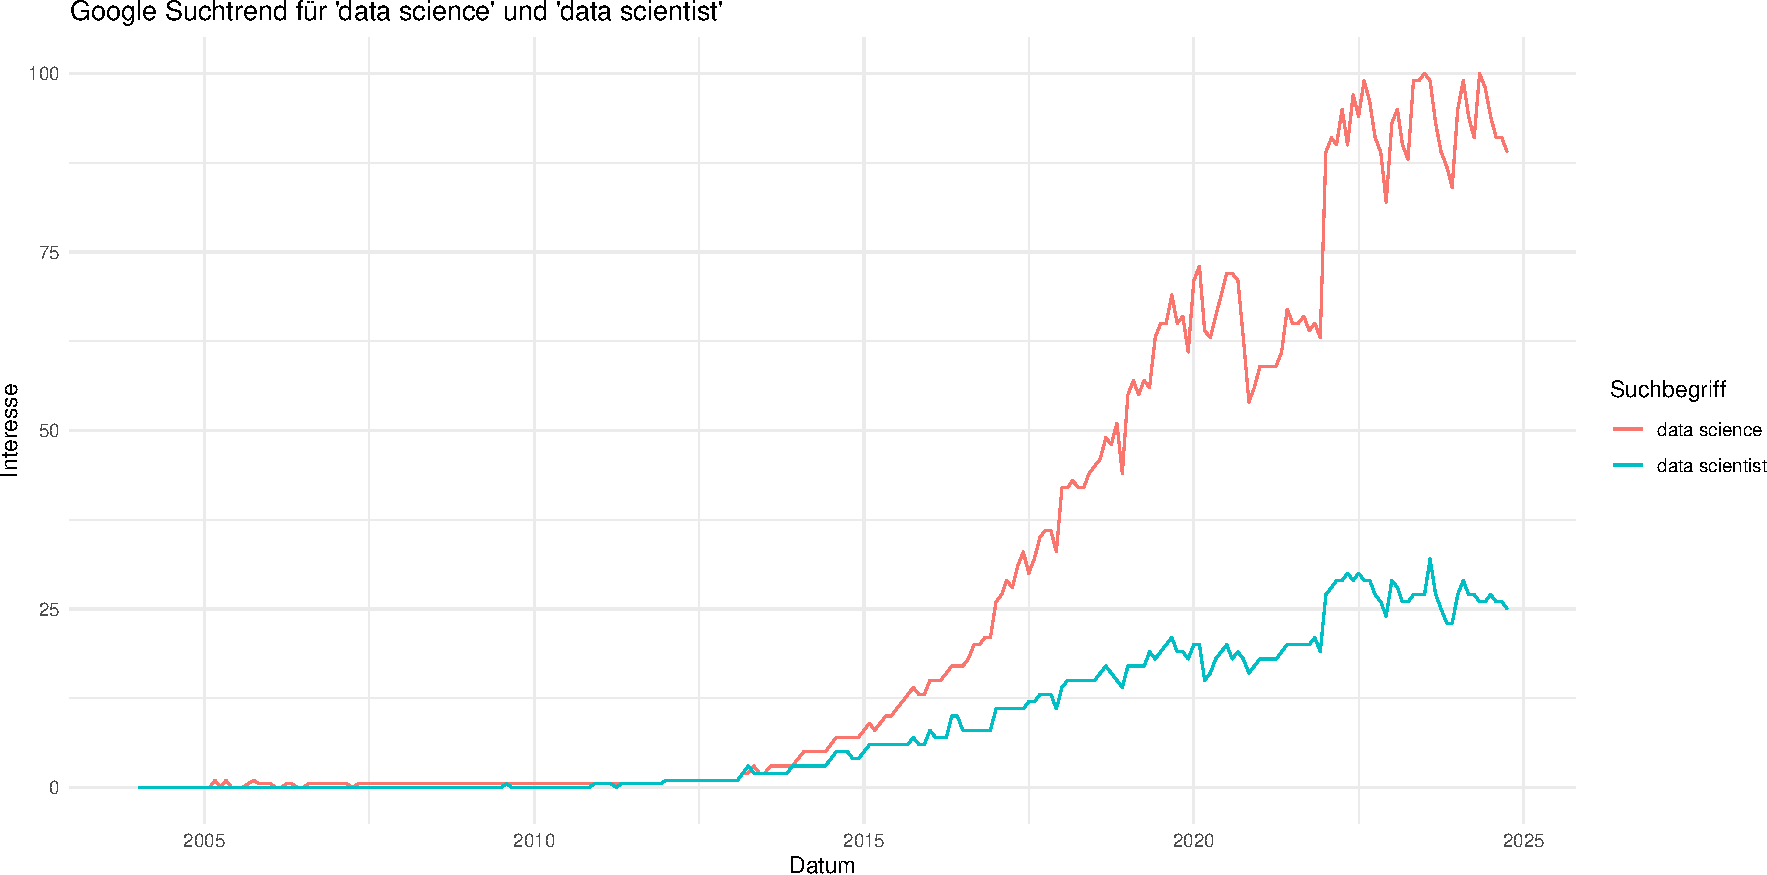
\includegraphics[keepaspectratio]{DataScience_files/figure-latex/unnamed-chunk-3-1.pdf}}

Das wachsende Interesse an Data Science stellt eine große Chance für
Arbeitnehmer dar. Ziel dieser Arbeit ist es einen Überblick über den
Data-Science-Jobmarkt zu geben, um Arbeitnehmern bei der Jobsuche zu
helfen und andererseits einen Überblick über die Gehälter und die Rolle
von Geographie und Wettbewerb bei Jobangeboten und Gehältern zu geben.

\subsection{Forschungsfrage}\label{forschungsfrage}

Im Rahmen der vorliegenden Arbeit wird die folgende Forschungsfrage
bearbeitet:

Inwiefern beeinflusst die geografische Nähe von Unternehmen das
Gehaltsniveau und die Verfügbarkeit von Data-Science-Jobs? Lässt sich
eine signifikante Variation der Einkommen innerhalb regionaler Cluster
feststellen, und wie kann diese durch Netzwerkzentralität erklärt
werden?

Zur Beantwortung dieser Forschungsfrage soll zudem analysiert werden,
inwiefern das Wettbewerbsumfeld zwischen Unternehmen die Gehaltsstruktur
im Bereich Data Science beeinflusst und welche Rolle zentrale
Unternehmen bei der Bestimmung des Gehaltsniveaus spielen.

\subsection{Datengrundlage}\label{datengrundlage}

Nachdem die Daten in Python extern als Vorbereitung aufbereitet wurden,
kann nun die Datengrundlage für diese Arbeit in R eingelesen werden.
Dabei wurde sich an
\url{https://www.kaggle.com/code/maxzeitler/data-science-job-salary-prediction-glassdoor/edit}
orientiert.

\subsubsection{CSV einlesen}\label{csv-einlesen}

\begin{Shaded}
\begin{Highlighting}[]
\NormalTok{data }\OtherTok{\textless{}{-}} \FunctionTok{read\_csv}\NormalTok{(}\StringTok{"data/Glassdoor\_DataScience\_Salary.csv"}\NormalTok{)}
\end{Highlighting}
\end{Shaded}

\begin{verbatim}
## Rows: 742 Columns: 28
## -- Column specification --------------------------------------------------------
## Delimiter: ","
## chr (14): Job Title, Job Description, Company Name, Location, Headquarters, ...
## dbl (14): Salary Estimate, Rating, Founded, Min_Salary, Max_Salary, Same Sta...
## 
## i Use `spec()` to retrieve the full column specification for this data.
## i Specify the column types or set `show_col_types = FALSE` to quiet this message.
\end{verbatim}

Die vorliegende Arbeit basiert auf einem Datensatz, der von Kaggle
stammt und Informationen zu Data-Science-Jobs in verschiedenen
Unternehmen enthält. Der Datensatz umfasst 742 Zeilen und 28 Spalten,
was auf eine Anzahl von 742 verschiedenen Jobangeboten hindeutet. Diese
Anzahl ist kann für die Zwecke dieser Arbeit als ausreichend zu
betrachten, auch wenn eine höhere Zahl an Beobachtungen möglicherweise
zu präziseren Schlussfolgerungen geführt hätte.

Der Datensatz beruht auf Daten, die von Glassdoor extrahiert wurden,
eine für Stellenanzeigen und Unternehmensbewertung bekannte Website, und
bietet detaillierte Informationen über Data-Science-Jobs sowie deren
Gehälter. Der Datensatz beinhaltet wesentliche Informationen, darunter
Jobtitel, geschätzte Gehälter, Stellenbeschreibungen,
Unternehmensbewertungen sowie relevante Unternehmensdaten wie Standort,
Größe und Branche. Eine detaillierte Beschreibung dieser Daten erfolgt
im späteren Verlauf. Der Datensatz eignet sich in besonderem Maße für
den Zweck dieser Arbeit, aber auch für Analysen des Arbeitsmarktes,
beispielsweise zur Untersuchung von Gehaltstrends oder zur
Identifizierung der am besten bewerteten Unternehmen.

Der Datensatz umfasst konkret die folgenden Spalten:

\subsubsection{Erste Ansicht der Daten}\label{erste-ansicht-der-daten}

\begin{Shaded}
\begin{Highlighting}[]
\FunctionTok{head}\NormalTok{(data, }\DecValTok{5}\NormalTok{)}
\end{Highlighting}
\end{Shaded}

\begin{verbatim}
## # A tibble: 5 x 28
##   `Job Title` `Salary Estimate` `Job Description` Rating `Company Name` Location
##   <chr>                   <dbl> <chr>              <dbl> <chr>          <chr>   
## 1 Data Scien~              72   "Data Scientist\~    3.8 Tecolote Rese~ Albuque~
## 2 Healthcare~              87.5 "What You Will D~    3.4 University of~ Linthic~
## 3 Data Scien~              85   "KnowBe4, Inc. i~    4.8 KnowBe4        Clearwa~
## 4 Data Scien~              76.5 "*Organization a~    3.8 PNNL           Richlan~
## 5 Data Scien~             114.  "Data Scientist\~    2.9 Affinity Solu~ New Yor~
## # i 22 more variables: Headquarters <chr>, Size <chr>, Founded <dbl>,
## #   `Type of ownership` <chr>, Industry <chr>, Sector <chr>, Revenue <chr>,
## #   Competitors <chr>, Min_Salary <dbl>, Max_Salary <dbl>, State <chr>,
## #   `Same State` <dbl>, Age <dbl>, Python_yn <dbl>, `R Studio` <dbl>,
## #   Spark <dbl>, AWS_yn <dbl>, Excel_yn <dbl>, Job_simp <chr>, job_state <chr>,
## #   desc_len <dbl>, Num_comp <dbl>
\end{verbatim}

\begin{Shaded}
\begin{Highlighting}[]
\FunctionTok{spec}\NormalTok{(data)}
\end{Highlighting}
\end{Shaded}

\begin{verbatim}
## cols(
##   `Job Title` = col_character(),
##   `Salary Estimate` = col_double(),
##   `Job Description` = col_character(),
##   Rating = col_double(),
##   `Company Name` = col_character(),
##   Location = col_character(),
##   Headquarters = col_character(),
##   Size = col_character(),
##   Founded = col_double(),
##   `Type of ownership` = col_character(),
##   Industry = col_character(),
##   Sector = col_character(),
##   Revenue = col_character(),
##   Competitors = col_character(),
##   Min_Salary = col_double(),
##   Max_Salary = col_double(),
##   State = col_character(),
##   `Same State` = col_double(),
##   Age = col_double(),
##   Python_yn = col_double(),
##   `R Studio` = col_double(),
##   Spark = col_double(),
##   AWS_yn = col_double(),
##   Excel_yn = col_double(),
##   Job_simp = col_character(),
##   job_state = col_character(),
##   desc_len = col_double(),
##   Num_comp = col_double()
## )
\end{verbatim}

\begin{Shaded}
\begin{Highlighting}[]
\FunctionTok{summary}\NormalTok{(data)}
\end{Highlighting}
\end{Shaded}

\begin{verbatim}
##   Job Title         Salary Estimate Job Description        Rating      
##  Length:742         Min.   : 13.5   Length:742         Min.   :-1.000  
##  Class :character   1st Qu.: 73.5   Class :character   1st Qu.: 3.300  
##  Mode  :character   Median : 97.5   Mode  :character   Median : 3.700  
##                     Mean   :100.6                      Mean   : 3.619  
##                     3rd Qu.:122.5                      3rd Qu.: 4.000  
##                     Max.   :254.0                      Max.   : 5.000  
##  Company Name         Location         Headquarters           Size          
##  Length:742         Length:742         Length:742         Length:742        
##  Class :character   Class :character   Class :character   Class :character  
##  Mode  :character   Mode  :character   Mode  :character   Mode  :character  
##                                                                             
##                                                                             
##                                                                             
##     Founded     Type of ownership    Industry            Sector         
##  Min.   :  -1   Length:742         Length:742         Length:742        
##  1st Qu.:1939   Class :character   Class :character   Class :character  
##  Median :1988   Mode  :character   Mode  :character   Mode  :character  
##  Mean   :1837                                                           
##  3rd Qu.:2007                                                           
##  Max.   :2019                                                           
##    Revenue          Competitors          Min_Salary       Max_Salary   
##  Length:742         Length:742         Min.   : 15.00   Min.   : 16.0  
##  Class :character   Class :character   1st Qu.: 52.00   1st Qu.: 96.0  
##  Mode  :character   Mode  :character   Median : 69.50   Median :124.0  
##                                        Mean   : 74.72   Mean   :127.2  
##                                        3rd Qu.: 91.00   3rd Qu.:155.0  
##                                        Max.   :202.00   Max.   :306.0  
##     State             Same State         Age           Python_yn     
##  Length:742         Min.   :0.000   Min.   : -1.00   Min.   :0.0000  
##  Class :character   1st Qu.:0.000   1st Qu.: 14.00   1st Qu.:0.0000  
##  Mode  :character   Median :1.000   Median : 27.00   Median :1.0000  
##                     Mean   :0.558   Mean   : 49.39   Mean   :0.5283  
##                     3rd Qu.:1.000   3rd Qu.: 62.00   3rd Qu.:1.0000  
##                     Max.   :1.000   Max.   :279.00   Max.   :1.0000  
##     R Studio            Spark            AWS_yn          Excel_yn     
##  Min.   :0.000000   Min.   :0.0000   Min.   :0.0000   Min.   :0.0000  
##  1st Qu.:0.000000   1st Qu.:0.0000   1st Qu.:0.0000   1st Qu.:0.0000  
##  Median :0.000000   Median :0.0000   Median :0.0000   Median :1.0000  
##  Mean   :0.002695   Mean   :0.2251   Mean   :0.2372   Mean   :0.5229  
##  3rd Qu.:0.000000   3rd Qu.:0.0000   3rd Qu.:0.0000   3rd Qu.:1.0000  
##  Max.   :1.000000   Max.   :1.0000   Max.   :1.0000   Max.   :1.0000  
##    Job_simp          job_state            desc_len        Num_comp    
##  Length:742         Length:742         Min.   :  407   Min.   :0.000  
##  Class :character   Class :character   1st Qu.: 2801   1st Qu.:0.000  
##  Mode  :character   Mode  :character   Median : 3731   Median :0.000  
##                                        Mean   : 3870   Mean   :1.054  
##                                        3rd Qu.: 4740   3rd Qu.:3.000  
##                                        Max.   :10051   Max.   :4.000
\end{verbatim}

Im Folgenden wird eine Übersicht der wesentlichen Spalten präsentiert:

\begin{itemize}
\tightlist
\item
  \texttt{Job\ Title}: Die Berufsbezeichnung, sie gibt Aufschluss über
  die Tätigkeit.
\item
  \texttt{Salary\ Estimate}: Die geschätzte Gehalt, in tausend Dollar
  pro Jahr. Es basiert auf dem Durchschnitt von dem minimalen und
  maximalen Gehalt.
\item
  \texttt{Job\ Description}, \texttt{Job\_simp}: Die Beschreibung der
  Stelle, die Aufgaben und Anforderungen enthält. Auch die vereinfachte
  Version der Berufsbezeichnung.
\item
  \texttt{Rating}: Die Bewertung des Unternehmens, sie weist eine
  Spannbreite von 1 bis 5 auf, wobei die Bewertung ``-1'' bei jeder
  Spalte für fehlende Bewertungen steht.
\item
  \texttt{Company\ Name}, \texttt{Location}, \texttt{Headquarters},
  \texttt{Size}, \texttt{Founded}: Unternehmensbezogene Daten wie Name,
  Standort, Sitz, Größe und Gründungsjahr des Unternehmens.
\item
  \texttt{Type\ of\ ownership}, \texttt{Industry}, \texttt{Sector},
  \texttt{Revenue}: Weitere Unternehmensmerkmale, diese umfassen die
  Eigentumsart, die Branche, den Sektor sowie die Einnahmen.
\item
  \texttt{Competitors}: Die Wettbewerber des Unternehmens, die im
  Zusammenhang dieser Arbeit von besonderer Bedeutung sind.
\item
  Skills (\texttt{Python\_yn}, \texttt{R\ Studio}, \texttt{Spark},
  \texttt{AWS\_yn}, \texttt{Excel\_yn}): Spalten, aus denen hervorgeht,
  ob die betreffende Kompetenz in der Stellenbeschreibung verlangt wird
  (0 = nein, 1 = ja).
\item
  \texttt{Min\_salary}, \texttt{Max\_salary}: Minimale und maximale
  Gehaltsschätzungen.
\item
  \texttt{State}, \texttt{Same\ State}, \texttt{job\_state},
  \texttt{Age}, \texttt{desc\_len}, \texttt{Num\_comp}: Zusätzliche
  Informationen wie Standort der Stelle, Alter des Unternehmens, Länge
  der Stellenbeschreibung und Anzahl der Mitbewerber.
\end{itemize}

Es zeigt sich, dass eine Vielzahl von Spalten für die vorliegende
Untersuchung irrelevant ist. Infolgedessen werden in einem späteren Teil
der Arbeit irrelevante Spalten, wie beispielsweise die Kenntnisse in
Python, R Studio, Spark und ähnlichen Programmen, welche ursprünglich
aus der Jobbeschreibung extrahiert wurden, entfernt.

Nachdem die Daten in Python mit Hilfe von Pandas bereinigt, ergänzt und
bearbeitet wurden, können sie nun in R eingelesen werden. Dabei wurde
sich an
\url{https://www.kaggle.com/code/maxzeitler/data-science-job-salary-prediction-glassdoor/edit}
orientiert.

Im Folgenden wird eine erste Betrachtung der Daten vorgenommen. Zu
diesem Zweck werden die Jobs in Florida nach ihren jeweiligen
Vergütungen geordnet und in Form eines Balkendiagramms dargestellt.

\begin{Shaded}
\begin{Highlighting}[]
\CommentTok{\# Filter data for the state of New York (NY)}
\NormalTok{data\_ny }\OtherTok{\textless{}{-}}\NormalTok{ data }\SpecialCharTok{\%\textgreater{}\%}
  \FunctionTok{filter}\NormalTok{(State }\SpecialCharTok{==} \StringTok{"NY"}\NormalTok{)}

\CommentTok{\# Calculate average salary by job title for NY}
\NormalTok{avg\_salary\_by\_job\_ny }\OtherTok{\textless{}{-}}\NormalTok{ data\_ny }\SpecialCharTok{\%\textgreater{}\%}
  \FunctionTok{group\_by}\NormalTok{(}\StringTok{\textasciigrave{}}\AttributeTok{Job Title}\StringTok{\textasciigrave{}}\NormalTok{) }\SpecialCharTok{\%\textgreater{}\%}
  \FunctionTok{summarise}\NormalTok{(}\AttributeTok{Average\_Salary =} \FunctionTok{mean}\NormalTok{(}\StringTok{\textasciigrave{}}\AttributeTok{Salary Estimate}\StringTok{\textasciigrave{}}\NormalTok{, }\AttributeTok{na.rm =} \ConstantTok{TRUE}\NormalTok{)) }\SpecialCharTok{\%\textgreater{}\%}
  \FunctionTok{arrange}\NormalTok{(}\FunctionTok{desc}\NormalTok{(Average\_Salary))}

\CommentTok{\# Bar plot of average salary by job title for NY}
\FunctionTok{ggplot}\NormalTok{(avg\_salary\_by\_job\_ny, }\FunctionTok{aes}\NormalTok{(}\AttributeTok{x =} \FunctionTok{reorder}\NormalTok{(}\StringTok{\textasciigrave{}}\AttributeTok{Job Title}\StringTok{\textasciigrave{}}\NormalTok{, Average\_Salary), }\AttributeTok{y =}\NormalTok{ Average\_Salary)) }\SpecialCharTok{+}
  \FunctionTok{geom\_bar}\NormalTok{(}\AttributeTok{stat =} \StringTok{"identity"}\NormalTok{) }\SpecialCharTok{+}
  \FunctionTok{coord\_flip}\NormalTok{() }\SpecialCharTok{+}
  \FunctionTok{labs}\NormalTok{(}\AttributeTok{title =} \StringTok{"Average Salary by Job Title in NY"}\NormalTok{, }\AttributeTok{x =} \StringTok{"Job Title"}\NormalTok{, }\AttributeTok{y =} \StringTok{"Average Salary"}\NormalTok{) }\SpecialCharTok{+}
  \FunctionTok{theme\_minimal}\NormalTok{() }\SpecialCharTok{+}
  \FunctionTok{theme}\NormalTok{(}
    \AttributeTok{axis.title =} \FunctionTok{element\_text}\NormalTok{(}\AttributeTok{size =} \DecValTok{14}\NormalTok{),}
    \AttributeTok{axis.text =} \FunctionTok{element\_text}\NormalTok{(}\AttributeTok{size =} \DecValTok{12}\NormalTok{),}
    \AttributeTok{plot.title =} \FunctionTok{element\_text}\NormalTok{(}\AttributeTok{size =} \DecValTok{16}\NormalTok{, }\AttributeTok{face =} \StringTok{"bold"}\NormalTok{)}
\NormalTok{  )}
\end{Highlighting}
\end{Shaded}

\pandocbounded{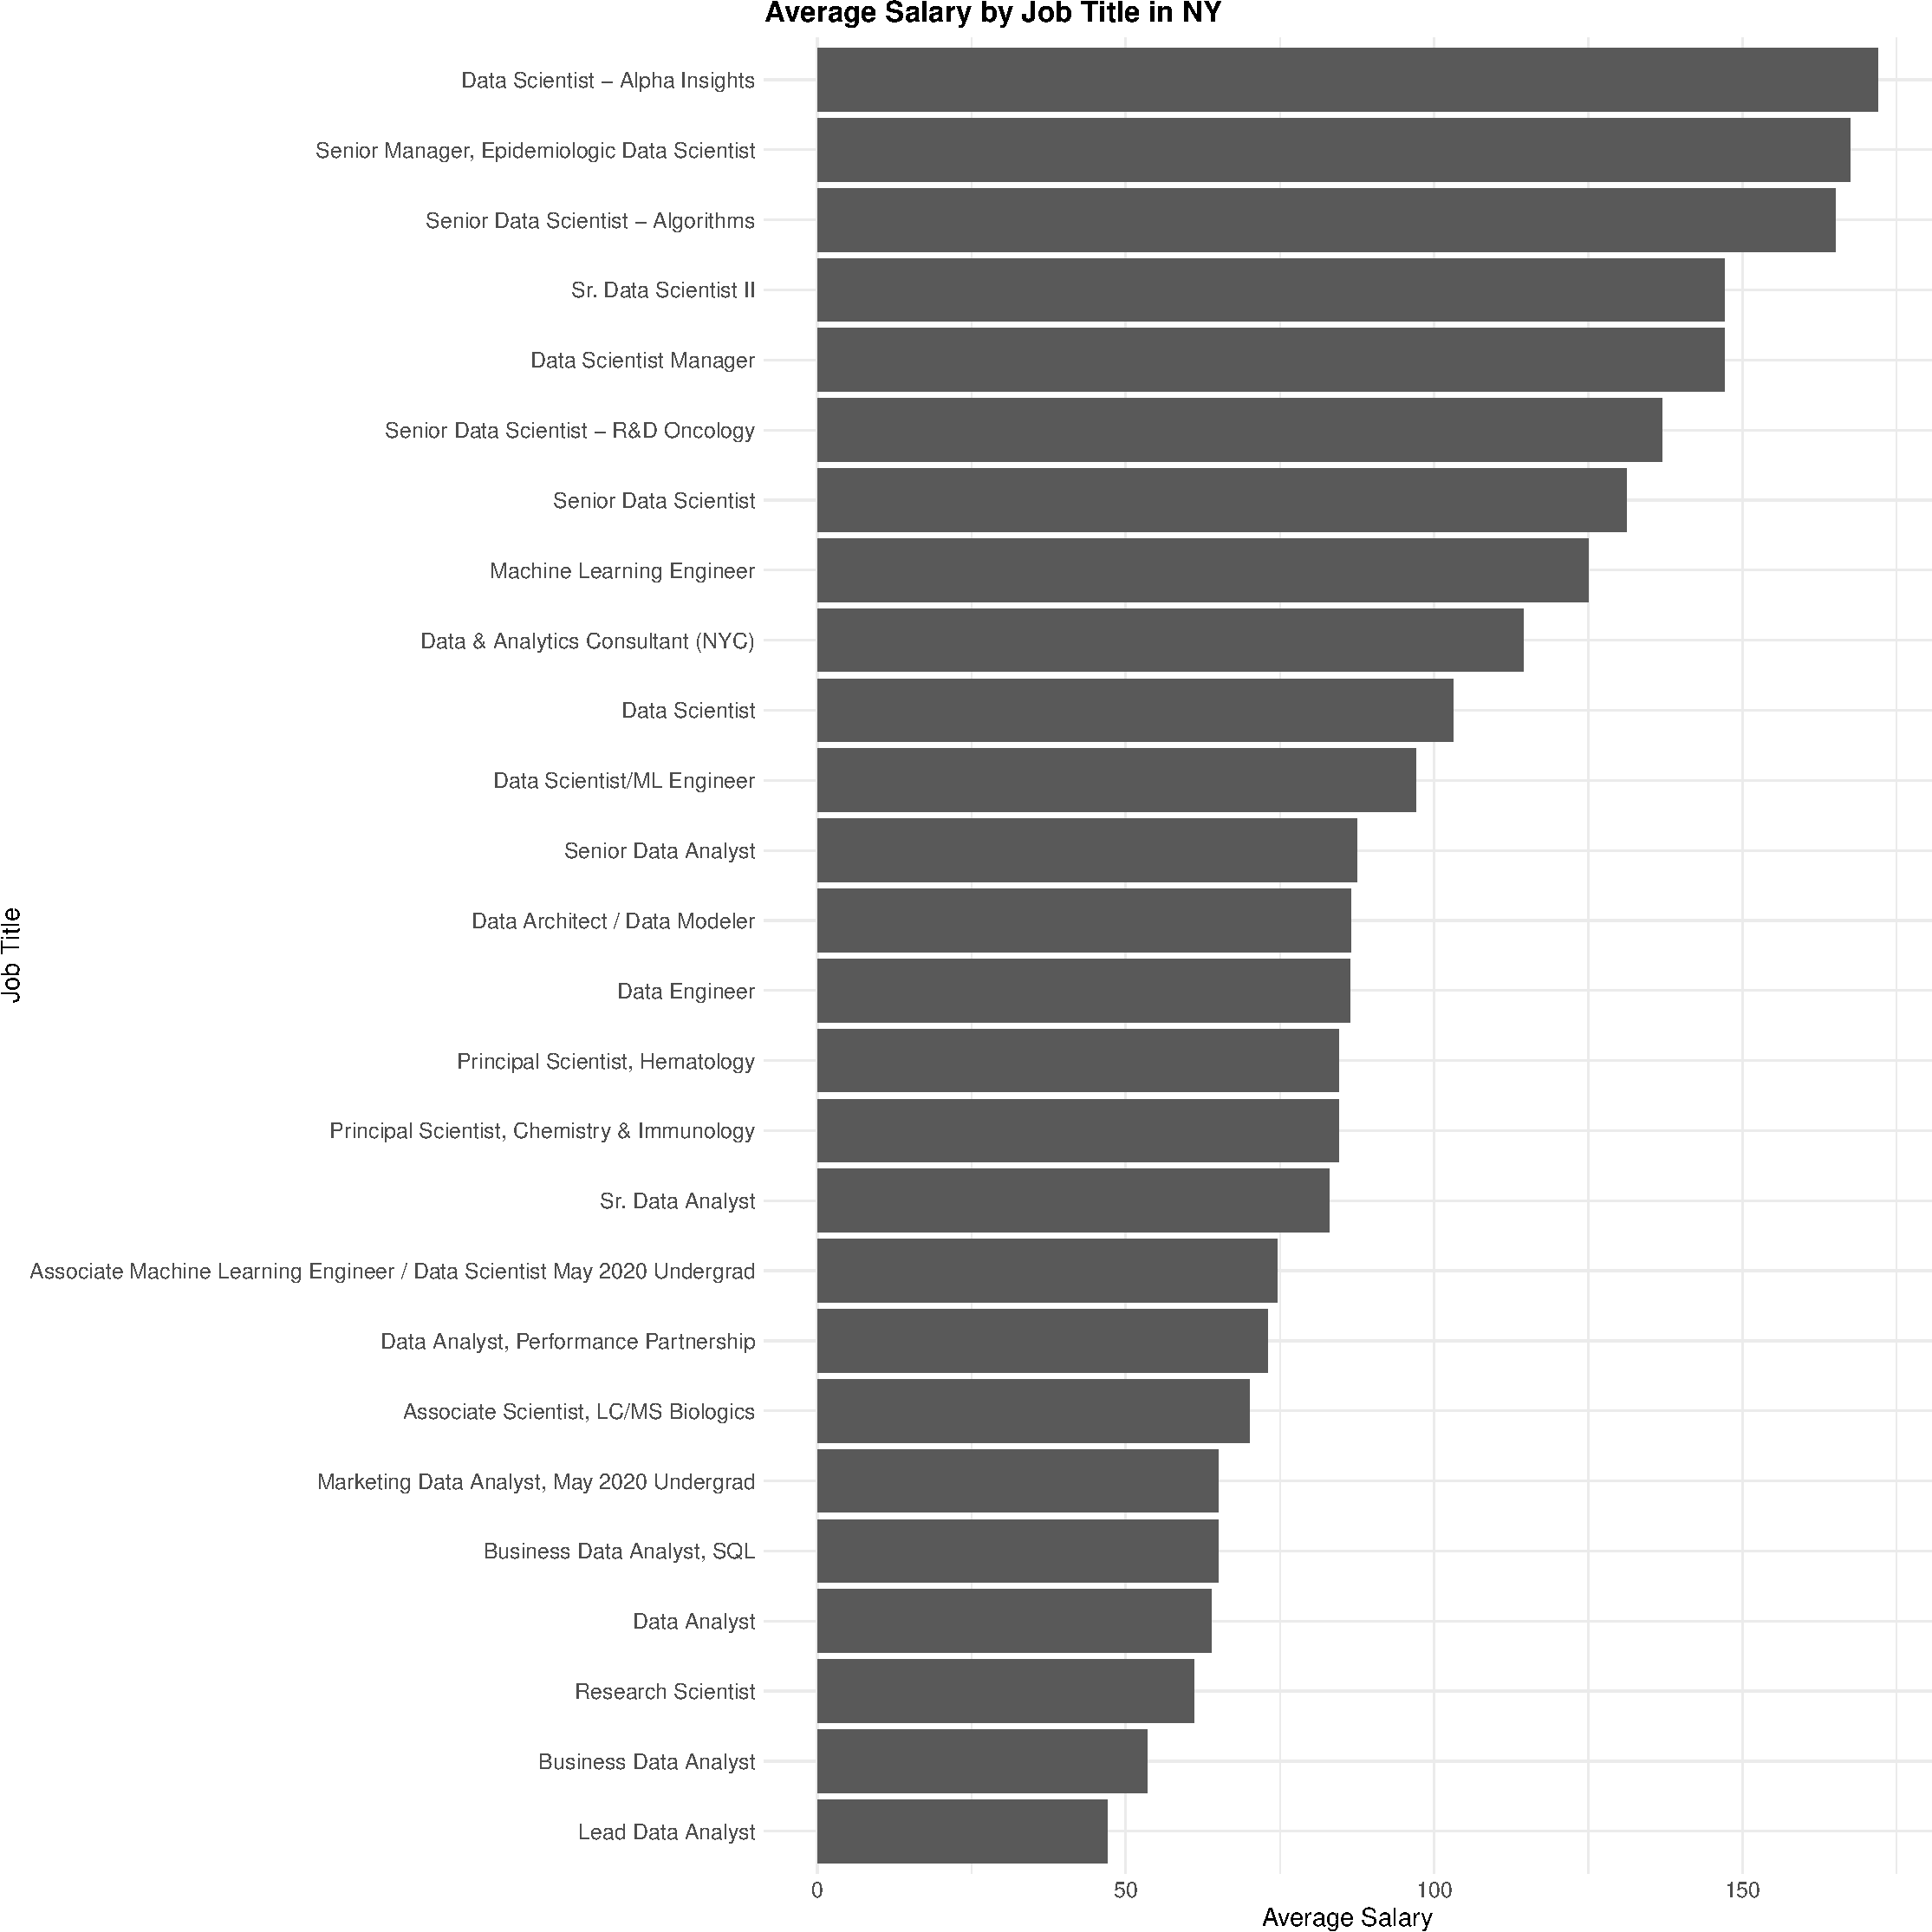
\includegraphics[keepaspectratio]{DataScience_files/figure-latex/unnamed-chunk-6-1.pdf}}

Kanten und Knoten ergänzen

\section{Analysestrategie}\label{analysestrategie}

\begin{enumerate}
\def\labelenumi{\arabic{enumi}.}
\tightlist
\item
  Geografisches Netzwerk
\end{enumerate}

Das Ziel besteht in der Erstellung eines Netzwerkes, welches auf der
räumlichen Nähe von Unternehmen basiert. Auf diese Weise soll untersucht
werden, inwiefern regional bedingte Faktoren die Gehälter beeinflussen.
Die Bildung von Kanten erfolgt nach dem Kriterium der räumlichen Nähe.
Dabei werden Unternehmen, die im gleichen Ort angesiedelt sind, durch
Kanten verbunden.

\begin{enumerate}
\def\labelenumi{\arabic{enumi}.}
\setcounter{enumi}{1}
\tightlist
\item
  Wettbewerbsnetzwerk
\end{enumerate}

Die vorliegende Untersuchung zielt darauf ab, den Einfluss des
Wettbewerbs auf die Gestaltung von Gehaltsstrukturen zu analysieren.
Dazu werden die Beziehungen zwischen konkurrierenden Unternehmen als
Netzwerk dargestellt. Die Bildung von Kanten durch Konkurrenzen erfolgt
wie folgt: Die in der Spalte ``Competitors'' gelisteten Unternehmen
werden als Knoten verbunden. In Bezug auf die Gewichtung sind
verschiedene Optionen denkbar. Beispielsweise könnte die direkte
Konkurrenz mit dem Wert ``1'' und die indirekte Konkurrenz mit dem Wert
``0,5'' bewertet werden. Dabei würde die indirekte Konkurrenz eine
Branche umfassen, in der das Unternehmen zwar nicht als direkter
Konkurrent aufgeführt ist, jedoch potenziell in Konkurrenz stehen
könnte. Im Rahmen der Netzwerkmetriken erfolgt eine Analyse der
folgenden Aspekte: Im Rahmen der Analyse von hierarchischen Beziehungen
und unterschiedlichen Zentralitäten erfolgt eine Untersuchung der
Wichtigkeit eines Unternehmens im Wettbewerbsnetzwerk sowie der
Gehaltshöhen in Relation zur Konkurrenz.

\begin{enumerate}
\def\labelenumi{\arabic{enumi}.}
\setcounter{enumi}{2}
\tightlist
\item
  Vergleich der Gehälter innerhalb der Netzwerke
\end{enumerate}

Im Rahmen der Analyse werden die Gehälter innerhalb der beiden Netzwerke
miteinander verglichen. Ziel ist die Identifikation von Unternehmen, die
zentral in einem der beiden Netzwerke liegen, und solchen, die am Rand
oder isoliert sind, um festzustellen, ob die zentralen Unternehmen
höhere Gehälter anbieten. Zur Durchführung des Gehaltsvergleichs werden
Korrelationen zwischen dem Gehalt und verschiedenen Zentralitätsmaßen
innerhalb der geografischen und wettbewerbsbezogenen Netzwerke
herangezogen. Darüber hinaus werden Cluster-Analysen durchgeführt, um
Unternehmen, die geografisch und wettbewerbsbedingt vernetzt sind,
miteinander zu vergleichen.

\begin{enumerate}
\def\labelenumi{\arabic{enumi}.}
\setcounter{enumi}{3}
\tightlist
\item
  Zusammenführung und Vergleich der Netzwerke
\end{enumerate}

Im Rahmen der Zusammenführung und des Vergleichs der Netzwerke erfolgt
eine Gegenüberstellung der jeweiligen Strukturen, um etwaige
Gemeinsamkeiten und Unterschiede zu identifizieren. Das Ziel dieser
Untersuchung besteht in der Analyse der Interaktion beider Netzwerke
sowie der Identifikation von Regionen, in denen eine besonders hohe
Gehaltskonkurrenz zu beobachten ist. Im Rahmen des Vergleichs der
Netzwerke hinsichtlich der Gehälter und des Wettbewerbs erfolgt zunächst
eine Gegenüberstellung der Gehaltsverteilung in sogenannten
``Hotspot-Regionen'' und geografisch isolierten Regionen. Darüber hinaus
werden gemeinsame Unternehmen in beiden Netzwerken sowie die
Gehaltsstrukturen innerhalb der Überschneidungsbereiche analysiert.

\section{Analyse}\label{analyse}

\subsection{Datenbereinigung}\label{datenbereinigung}

Bei der Durchsicht des Datensatzes viel auf, dass die Spalten ``Same
State'' und ``job\_state'' von der Logik her ähnlich sind. Dies soll nun
näher unterucht werden, um spätere Fehler vorzubeugen.

\begin{Shaded}
\begin{Highlighting}[]
\CommentTok{\# Select "State" and "job\_state" columns}
\NormalTok{selected\_data }\OtherTok{\textless{}{-}}\NormalTok{ data }\SpecialCharTok{\%\textgreater{}\%}
  \FunctionTok{select}\NormalTok{(State, job\_state)}

\CommentTok{\# Display the first few rows of the selected data}
\FunctionTok{head}\NormalTok{(selected\_data, }\DecValTok{15}\NormalTok{)}
\end{Highlighting}
\end{Shaded}

\begin{verbatim}
## # A tibble: 15 x 2
##    State job_state
##    <chr> <chr>    
##  1 NM    NM       
##  2 MD    MD       
##  3 FL    FL       
##  4 WA    WA       
##  5 NY    NY       
##  6 TX    TX       
##  7 MD    MD       
##  8 CA    CA       
##  9 NY    NY       
## 10 NY    NY       
## 11 CA    CA       
## 12 VA    VA       
## 13 TX    TX       
## 14 WA    WA       
## 15 MA    MA
\end{verbatim}

Sieht so aus, als wäre beide Spalten identisch.

\begin{Shaded}
\begin{Highlighting}[]
\CommentTok{\# Check if the "State" and "job\_state" columns are identical}
\ControlFlowTok{if}\NormalTok{ (}\FunctionTok{all}\NormalTok{(selected\_data}\SpecialCharTok{$}\NormalTok{State }\SpecialCharTok{==}\NormalTok{ selected\_data}\SpecialCharTok{$}\NormalTok{job\_state, }\AttributeTok{na.rm =} \ConstantTok{TRUE}\NormalTok{)) \{}
  \FunctionTok{print}\NormalTok{(}\StringTok{"All values in \textquotesingle{}State\textquotesingle{} and \textquotesingle{}job\_state\textquotesingle{} columns are identical."}\NormalTok{)}
\NormalTok{\} }\ControlFlowTok{else}\NormalTok{ \{}
  \FunctionTok{print}\NormalTok{(}\StringTok{"There are differences between \textquotesingle{}State\textquotesingle{} and \textquotesingle{}job\_state\textquotesingle{} columns."}\NormalTok{)}
\NormalTok{\}}
\end{Highlighting}
\end{Shaded}

\begin{verbatim}
## [1] "There are differences between 'State' and 'job_state' columns."
\end{verbatim}

Jedoch trügt der Schein, da es Unterschiede gibt.

\begin{Shaded}
\begin{Highlighting}[]
\CommentTok{\# Filter rows where State is not equal to job\_state}
\NormalTok{different\_states }\OtherTok{\textless{}{-}}\NormalTok{ selected\_data }\SpecialCharTok{\%\textgreater{}\%}
  \FunctionTok{filter}\NormalTok{(State }\SpecialCharTok{!=}\NormalTok{ job\_state)}

\CommentTok{\# Display all rows where State is not equal to job\_state}
\FunctionTok{print}\NormalTok{(different\_states, }\AttributeTok{n =} \ConstantTok{Inf}\NormalTok{)}
\end{Highlighting}
\end{Shaded}

\begin{verbatim}
## # A tibble: 1 x 2
##   State       job_state
##   <chr>       <chr>    
## 1 Los Angeles CA
\end{verbatim}

Es fällt auf, das LA und Los Angeles nicht einheitlich verwendet werden.
Außerdem ist Los Angeles kein eigener Bundesstaat, sonder ein Teil von
Kalifornien(CA). Dies soll nun korrigiert werden.

Außerdem sollte bei weieren Vorgehen beachtet werden, dass Werte wie
``Na'' oder ``-1'' vor den Analysen entfernt werden sollten.

\begin{Shaded}
\begin{Highlighting}[]
\CommentTok{\# First step: Replace "Los Angeles" with "LA"}
\NormalTok{data }\OtherTok{\textless{}{-}}\NormalTok{ data }\SpecialCharTok{\%\textgreater{}\%}
  \FunctionTok{mutate}\NormalTok{(}\AttributeTok{State =} \FunctionTok{ifelse}\NormalTok{(State }\SpecialCharTok{==} \StringTok{"Los Angeles"}\NormalTok{, }\StringTok{"LA"}\NormalTok{, State),}
         \AttributeTok{job\_state =} \FunctionTok{ifelse}\NormalTok{(job\_state }\SpecialCharTok{==} \StringTok{"Los Angeles"}\NormalTok{, }\StringTok{"LA"}\NormalTok{, job\_state))}

\CommentTok{\# Second step: Replace "LA" with "CA"}
\NormalTok{data }\OtherTok{\textless{}{-}}\NormalTok{ data }\SpecialCharTok{\%\textgreater{}\%}
  \FunctionTok{mutate}\NormalTok{(}\AttributeTok{State =} \FunctionTok{ifelse}\NormalTok{(State }\SpecialCharTok{==} \StringTok{"LA"}\NormalTok{, }\StringTok{"CA"}\NormalTok{, State),}
         \AttributeTok{job\_state =} \FunctionTok{ifelse}\NormalTok{(job\_state }\SpecialCharTok{==} \StringTok{"LA"}\NormalTok{, }\StringTok{"CA"}\NormalTok{, job\_state))}

\CommentTok{\# Re{-}check for differences after correction}
\NormalTok{selected\_data }\OtherTok{\textless{}{-}}\NormalTok{ data }\SpecialCharTok{\%\textgreater{}\%}
  \FunctionTok{select}\NormalTok{(State, job\_state)}

\CommentTok{\# Check if the "State" and "job\_state" columns are identical}
\ControlFlowTok{if}\NormalTok{ (}\FunctionTok{all}\NormalTok{(selected\_data}\SpecialCharTok{$}\NormalTok{State }\SpecialCharTok{==}\NormalTok{ selected\_data}\SpecialCharTok{$}\NormalTok{job\_state, }\AttributeTok{na.rm =} \ConstantTok{TRUE}\NormalTok{)) \{}
  \FunctionTok{print}\NormalTok{(}\StringTok{"All values in \textquotesingle{}State\textquotesingle{} and \textquotesingle{}job\_state\textquotesingle{} columns are identical."}\NormalTok{)}
\NormalTok{\} }\ControlFlowTok{else}\NormalTok{ \{}
  \FunctionTok{print}\NormalTok{(}\StringTok{"There are differences between \textquotesingle{}State\textquotesingle{} and \textquotesingle{}job\_state\textquotesingle{} columns."}\NormalTok{)}
\NormalTok{\}}
\end{Highlighting}
\end{Shaded}

\begin{verbatim}
## [1] "All values in 'State' and 'job_state' columns are identical."
\end{verbatim}

\subsection{Visualisierung}\label{visualisierung}

\begin{Shaded}
\begin{Highlighting}[]
\CommentTok{\# AAus Gründen der Sichtbarkeit, werden bloß Locations mit mehr als einem Unternehmen dargestellt.}

\CommentTok{\# Extract relevant columns for geographic visualization}
\NormalTok{edges\_geo }\OtherTok{\textless{}{-}}\NormalTok{ data }\SpecialCharTok{\%\textgreater{}\%}
  \FunctionTok{select}\NormalTok{(}\AttributeTok{Company =} \StringTok{\textasciigrave{}}\AttributeTok{Company Name}\StringTok{\textasciigrave{}}\NormalTok{, }\AttributeTok{Location =} \StringTok{\textasciigrave{}}\AttributeTok{Location}\StringTok{\textasciigrave{}}\NormalTok{) }\SpecialCharTok{\%\textgreater{}\%}
  \FunctionTok{distinct}\NormalTok{()}

\CommentTok{\# Calculate the number of companies per location and filter for locations with more than one company}
\NormalTok{location\_counts }\OtherTok{\textless{}{-}}\NormalTok{ edges\_geo }\SpecialCharTok{\%\textgreater{}\%}
  \FunctionTok{group\_by}\NormalTok{(Location) }\SpecialCharTok{\%\textgreater{}\%}
  \FunctionTok{summarise}\NormalTok{(}\AttributeTok{Company\_Count =} \FunctionTok{n}\NormalTok{()) }\SpecialCharTok{\%\textgreater{}\%}
  \FunctionTok{filter}\NormalTok{(Company\_Count }\SpecialCharTok{\textgreater{}} \DecValTok{1}\NormalTok{)  }\CommentTok{\# Keep only locations with more than one company}

\CommentTok{\# Filter edges to include only connections for locations with more than one company}
\NormalTok{filtered\_edges }\OtherTok{\textless{}{-}}\NormalTok{ edges\_geo }\SpecialCharTok{\%\textgreater{}\%}
  \FunctionTok{filter}\NormalTok{(Location }\SpecialCharTok{\%in\%}\NormalTok{ location\_counts}\SpecialCharTok{$}\NormalTok{Location)}

\CommentTok{\# Create an igraph object for geographic visualization}
\NormalTok{network\_geo }\OtherTok{\textless{}{-}} \FunctionTok{graph\_from\_data\_frame}\NormalTok{(filtered\_edges, }\AttributeTok{directed =} \ConstantTok{FALSE}\NormalTok{)}

\CommentTok{\# Set vertex colors based on whether the node is a company or a location}
\NormalTok{company\_colors }\OtherTok{\textless{}{-}} \StringTok{"blue"}
\NormalTok{location\_colors }\OtherTok{\textless{}{-}} \FunctionTok{rainbow}\NormalTok{(}\FunctionTok{nrow}\NormalTok{(location\_counts))}

\CommentTok{\# Set vertex size based on the number of companies at each location}
\NormalTok{vertex\_sizes }\OtherTok{\textless{}{-}} \FunctionTok{ifelse}\NormalTok{(}\FunctionTok{V}\NormalTok{(network\_geo)}\SpecialCharTok{$}\NormalTok{name }\SpecialCharTok{\%in\%}\NormalTok{ location\_counts}\SpecialCharTok{$}\NormalTok{Location,}
                       \FunctionTok{sqrt}\NormalTok{(location\_counts}\SpecialCharTok{$}\NormalTok{Company\_Count[}\FunctionTok{match}\NormalTok{(}\FunctionTok{V}\NormalTok{(network\_geo)}\SpecialCharTok{$}\NormalTok{name, location\_counts}\SpecialCharTok{$}\NormalTok{Location)]) }\SpecialCharTok{*} \DecValTok{2}\NormalTok{,}
                       \DecValTok{3}\NormalTok{)  }\CommentTok{\# Default size for companies}

\CommentTok{\# Assign colors and sizes to vertices}
\FunctionTok{V}\NormalTok{(network\_geo)}\SpecialCharTok{$}\NormalTok{size }\OtherTok{\textless{}{-}}\NormalTok{ vertex\_sizes}
\FunctionTok{V}\NormalTok{(network\_geo)}\SpecialCharTok{$}\NormalTok{color }\OtherTok{\textless{}{-}} \FunctionTok{ifelse}\NormalTok{(}\FunctionTok{V}\NormalTok{(network\_geo)}\SpecialCharTok{$}\NormalTok{name }\SpecialCharTok{\%in\%}\NormalTok{ filtered\_edges}\SpecialCharTok{$}\NormalTok{Company, }
\NormalTok{                               company\_colors, }
                               \FunctionTok{ifelse}\NormalTok{(vertex\_sizes }\SpecialCharTok{\textgreater{}} \DecValTok{5}\NormalTok{, location\_colors[}\FunctionTok{match}\NormalTok{(}\FunctionTok{V}\NormalTok{(network\_geo)}\SpecialCharTok{$}\NormalTok{name, location\_counts}\SpecialCharTok{$}\NormalTok{Location)], }\StringTok{"grey"}\NormalTok{))}

\CommentTok{\# Plot the network}
\FunctionTok{plot}\NormalTok{(network\_geo, }
     \AttributeTok{vertex.label =} \ConstantTok{NA}\NormalTok{,  }\CommentTok{\# Remove labels from the plot}
     \AttributeTok{vertex.size =} \FunctionTok{V}\NormalTok{(network\_geo)}\SpecialCharTok{$}\NormalTok{size, }
     \AttributeTok{vertex.color =} \FunctionTok{V}\NormalTok{(network\_geo)}\SpecialCharTok{$}\NormalTok{color, }
     \AttributeTok{edge.arrow.size =} \FloatTok{0.3}\NormalTok{, }
     \AttributeTok{layout =}\NormalTok{ layout\_with\_fr, }
\NormalTok{)}

\CommentTok{\# Add legend for locations with size \textgreater{} 5}
\NormalTok{large\_locations }\OtherTok{\textless{}{-}}\NormalTok{ location\_counts}\SpecialCharTok{$}\NormalTok{Location[vertex\_sizes[}\FunctionTok{match}\NormalTok{(location\_counts}\SpecialCharTok{$}\NormalTok{Location, }\FunctionTok{V}\NormalTok{(network\_geo)}\SpecialCharTok{$}\NormalTok{name)] }\SpecialCharTok{\textgreater{}} \DecValTok{5}\NormalTok{]}
\NormalTok{large\_location\_colors }\OtherTok{\textless{}{-}}\NormalTok{ location\_colors[}\FunctionTok{match}\NormalTok{(large\_locations, location\_counts}\SpecialCharTok{$}\NormalTok{Location)]}
\FunctionTok{legend}\NormalTok{(}\StringTok{"topright"}\NormalTok{, }\AttributeTok{legend =}\NormalTok{ large\_locations, }\AttributeTok{col =}\NormalTok{ large\_location\_colors, }\AttributeTok{pch =} \DecValTok{19}\NormalTok{, }\AttributeTok{title =} \StringTok{"Locations"}\NormalTok{)}
\end{Highlighting}
\end{Shaded}

\pandocbounded{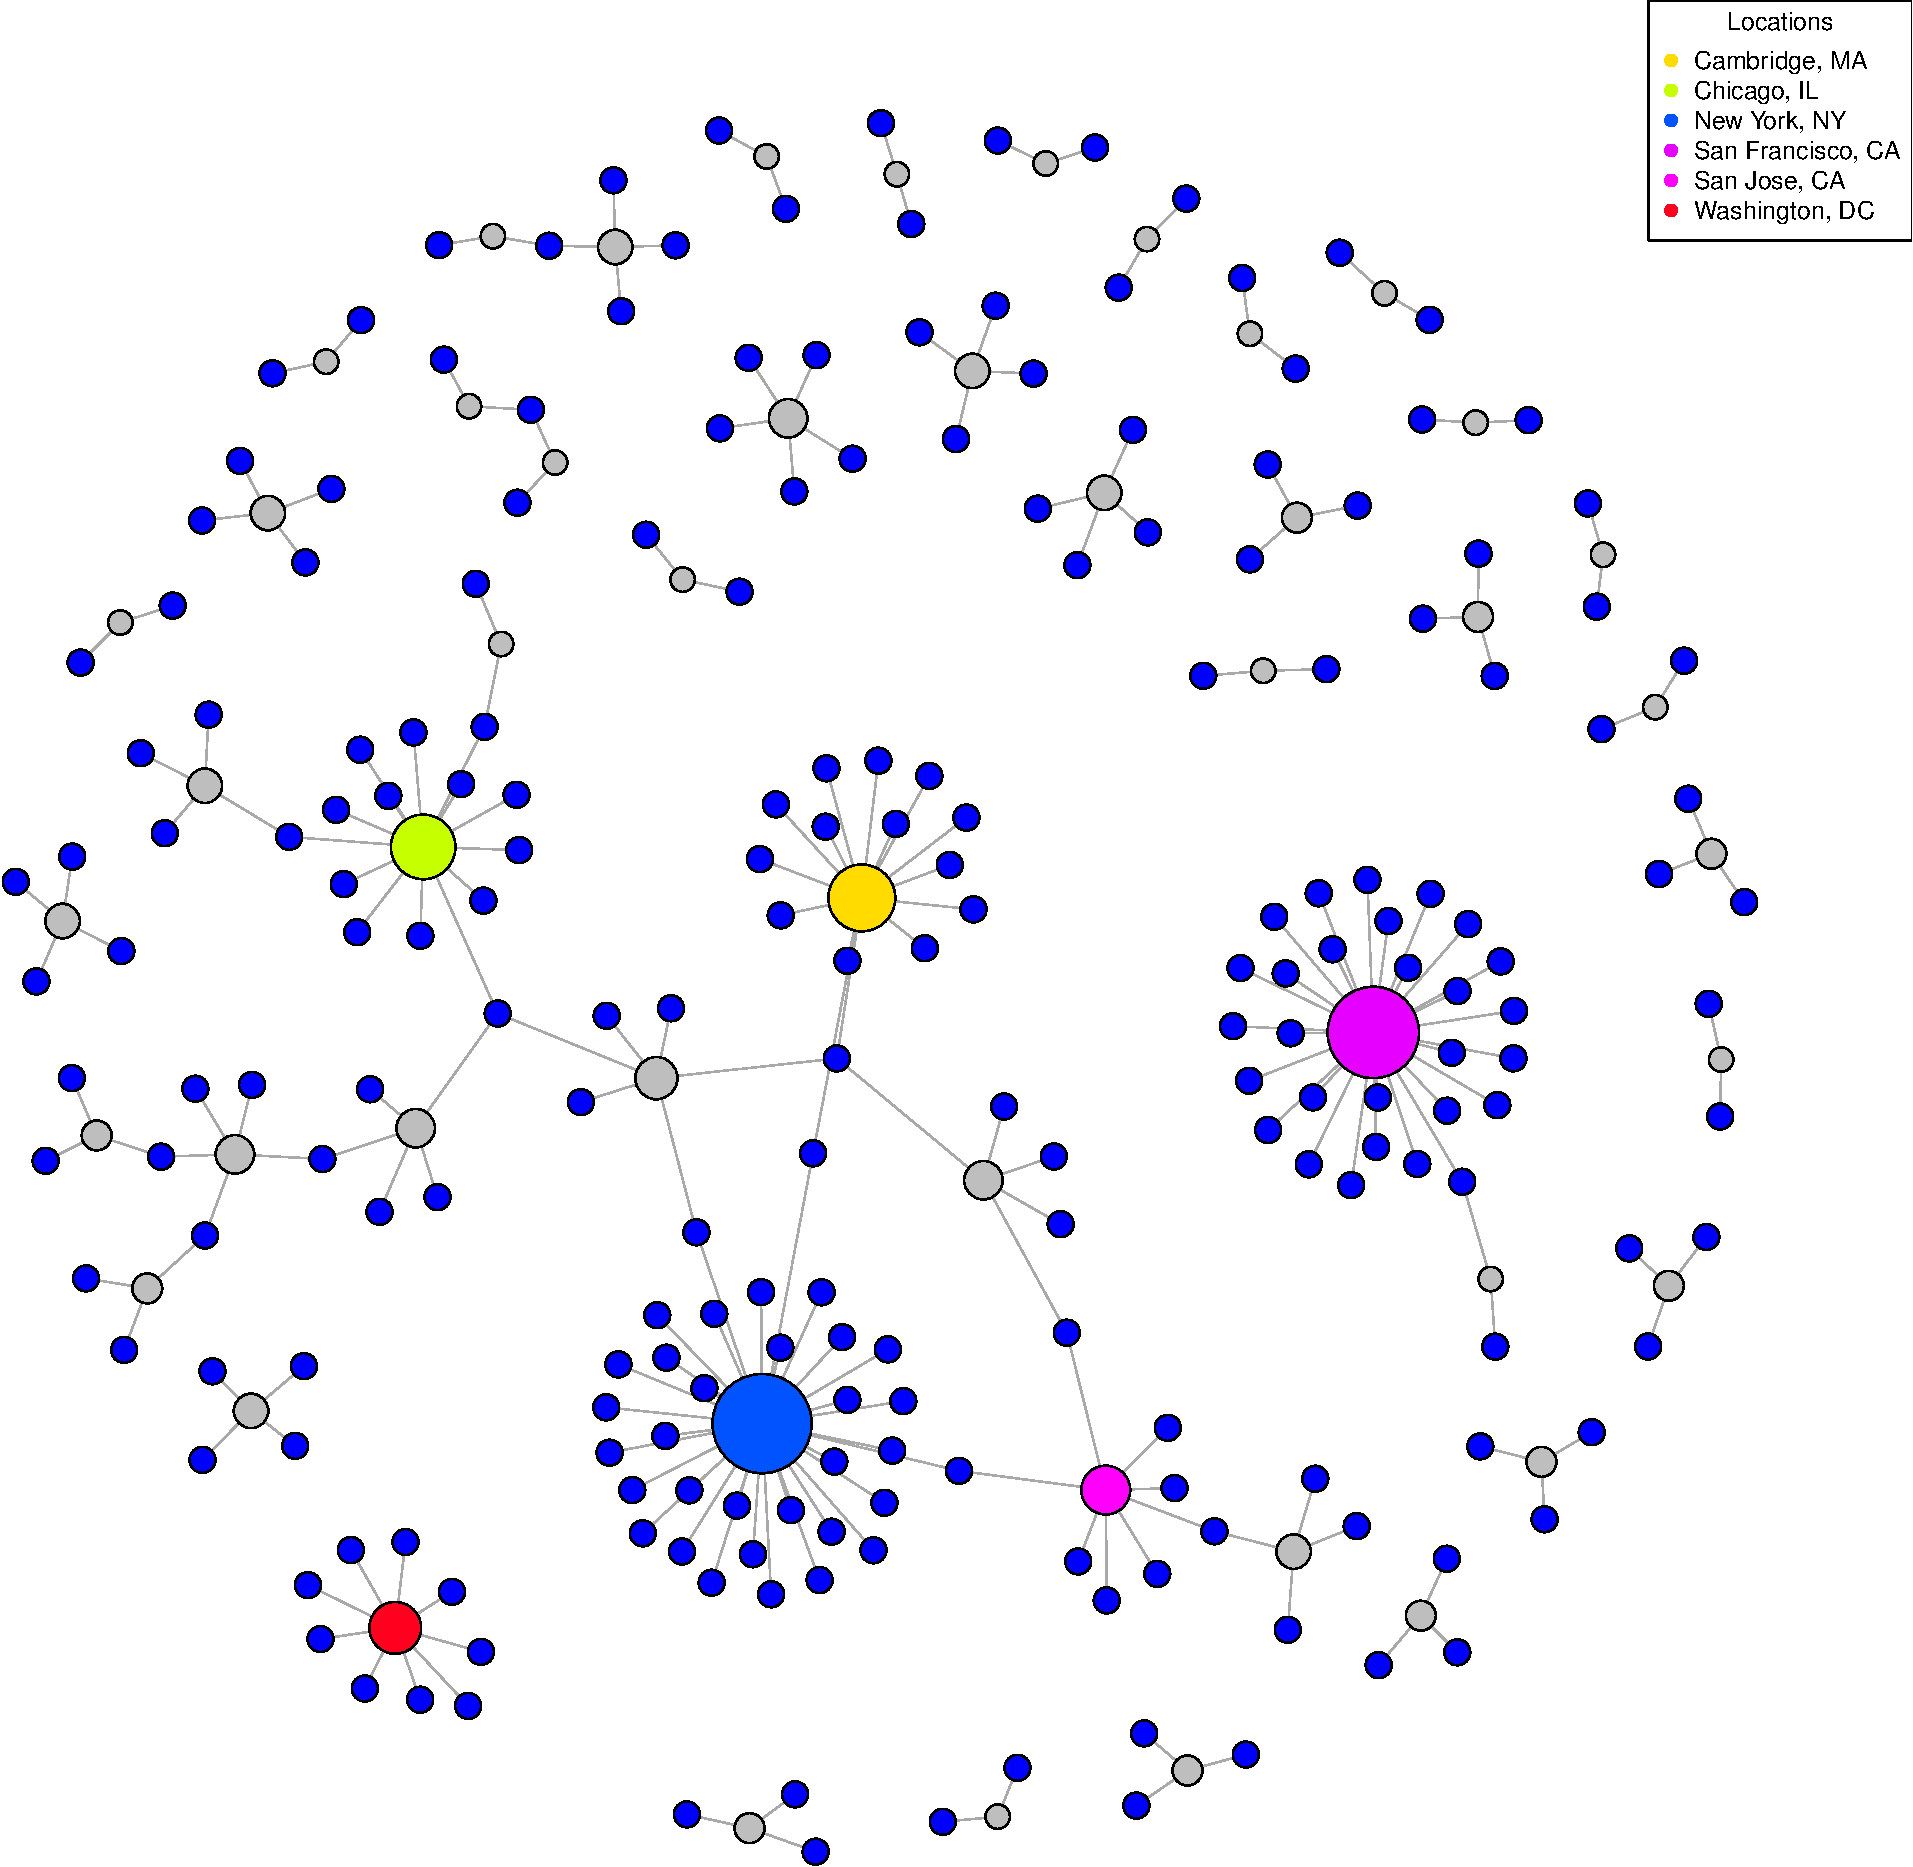
\includegraphics[keepaspectratio]{DataScience_files/figure-latex/unnamed-chunk-11-1.pdf}}

\subsection{Datenvisualisierung}\label{datenvisualisierung}

\#Netzwerk von Jobtiteln und Unternehmen: \#Visualisierung des
Netzwerks, das zeigt, welche Unternehmen die meisten unterschiedlichen
Jobtitel anbieten. \#Interpretation: Zentralität der Unternehmen und
welche Rolle sie im Jobmarkt spielen. \#Degree distribution

\begin{Shaded}
\begin{Highlighting}[]
\CommentTok{\# Create the network object}
\NormalTok{edges }\OtherTok{\textless{}{-}}\NormalTok{ data }\SpecialCharTok{\%\textgreater{}\%}
  \FunctionTok{select}\NormalTok{(}\StringTok{\textasciigrave{}}\AttributeTok{Job Title}\StringTok{\textasciigrave{}}\NormalTok{, }\StringTok{\textasciigrave{}}\AttributeTok{Company Name}\StringTok{\textasciigrave{}}\NormalTok{) }\SpecialCharTok{\%\textgreater{}\%}
  \FunctionTok{distinct}\NormalTok{() }\SpecialCharTok{\%\textgreater{}\%}
  \FunctionTok{rename}\NormalTok{(}\AttributeTok{from =} \StringTok{\textasciigrave{}}\AttributeTok{Job Title}\StringTok{\textasciigrave{}}\NormalTok{, }\AttributeTok{to =} \StringTok{\textasciigrave{}}\AttributeTok{Company Name}\StringTok{\textasciigrave{}}\NormalTok{)}

\NormalTok{network\_job\_company }\OtherTok{\textless{}{-}} \FunctionTok{graph\_from\_data\_frame}\NormalTok{(edges, }\AttributeTok{directed =} \ConstantTok{FALSE}\NormalTok{)}

\NormalTok{degree\_distribution }\OtherTok{\textless{}{-}} \FunctionTok{degree}\NormalTok{(network\_job\_company)}
\FunctionTok{hist}\NormalTok{(degree\_distribution, }\AttributeTok{breaks =} \DecValTok{30}\NormalTok{, }\AttributeTok{main =} \StringTok{"Degree Distribution"}\NormalTok{,}
     \AttributeTok{xlab =} \StringTok{"Degree"}\NormalTok{, }\AttributeTok{ylab =} \StringTok{"Frequency"}\NormalTok{)}
\end{Highlighting}
\end{Shaded}

\pandocbounded{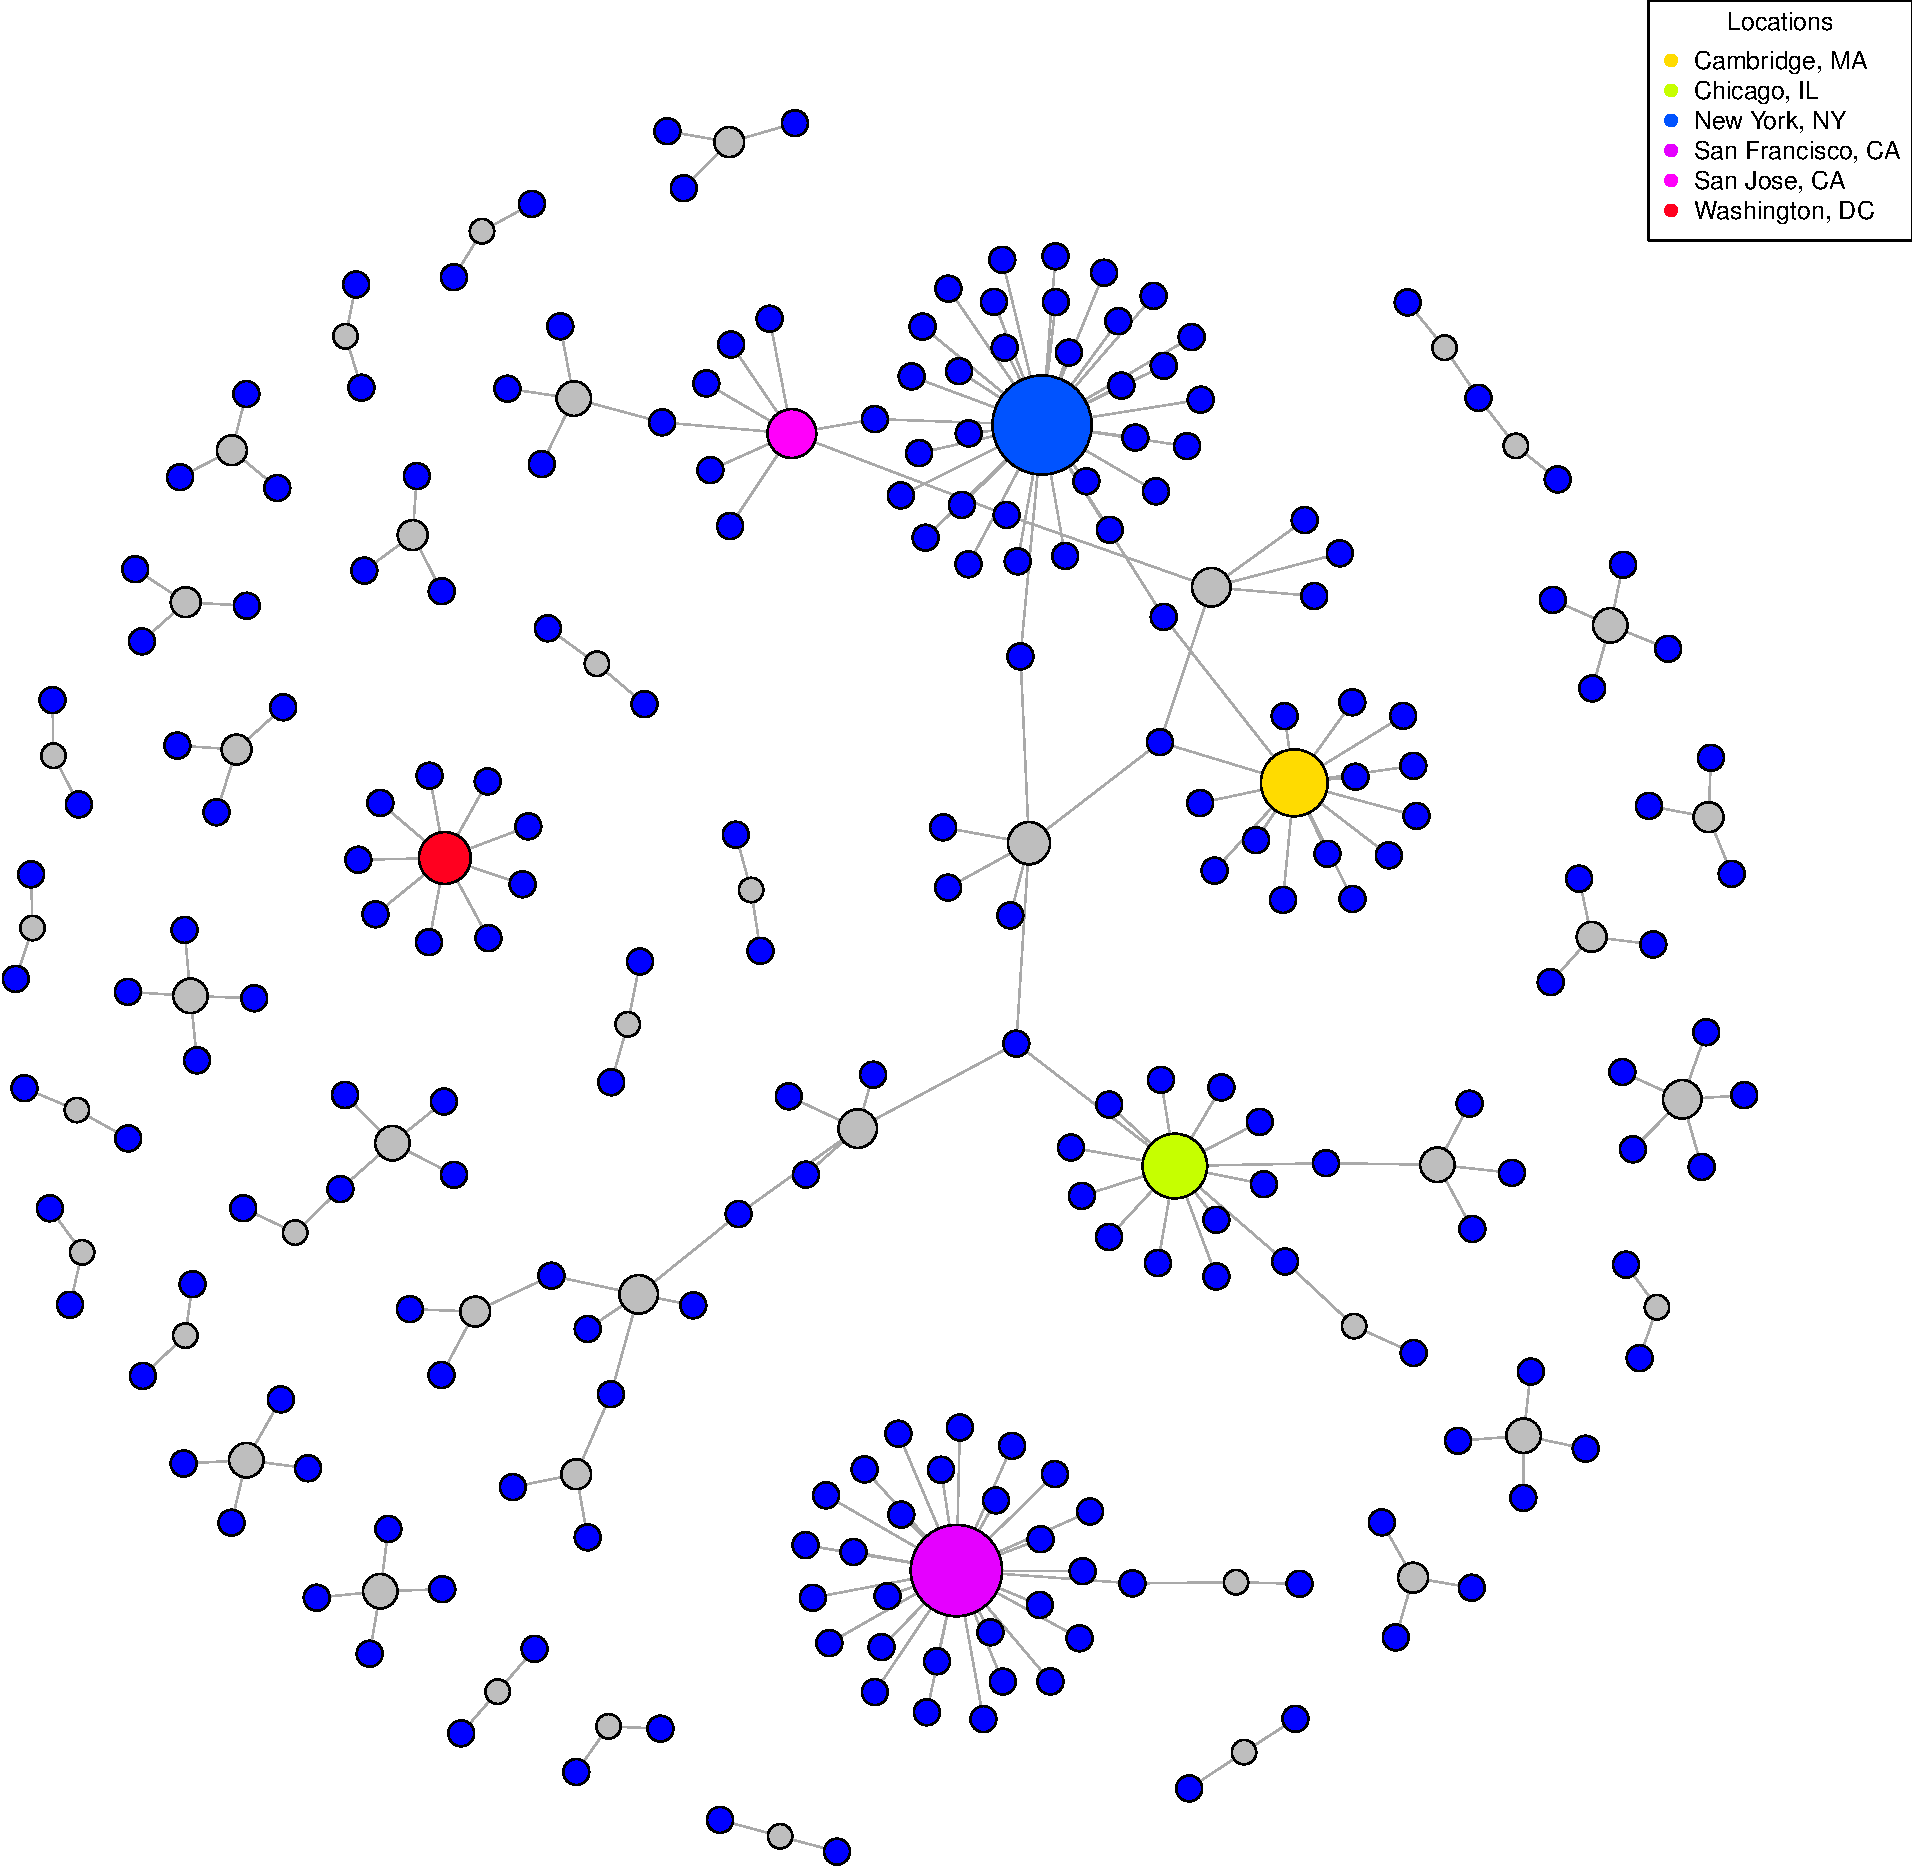
\includegraphics[keepaspectratio]{DataScience_files/figure-latex/unnamed-chunk-12-1.pdf}}

\begin{Shaded}
\begin{Highlighting}[]
\CommentTok{\# Community detection using the Louvain method}
\NormalTok{communities }\OtherTok{\textless{}{-}} \FunctionTok{cluster\_louvain}\NormalTok{(network\_job\_company)}
\FunctionTok{plot}\NormalTok{(network\_job\_company, }\AttributeTok{vertex.label =} \ConstantTok{NA}\NormalTok{, }\AttributeTok{vertex.size =} \DecValTok{5}\NormalTok{,}
     \AttributeTok{vertex.color =}\NormalTok{ communities}\SpecialCharTok{$}\NormalTok{membership)}
\end{Highlighting}
\end{Shaded}

\pandocbounded{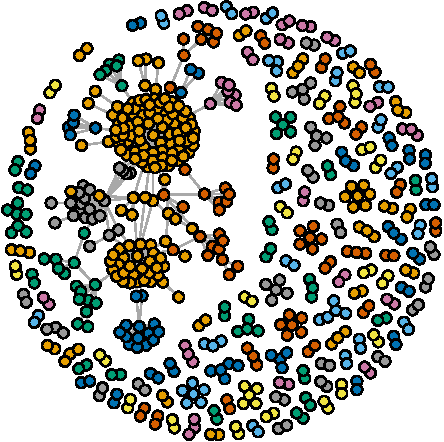
\includegraphics[keepaspectratio]{DataScience_files/figure-latex/unnamed-chunk-12-2.pdf}}

\begin{Shaded}
\begin{Highlighting}[]
\CommentTok{\# Calculate betweenness centrality}
\NormalTok{betweenness\_centrality }\OtherTok{\textless{}{-}} \FunctionTok{betweenness}\NormalTok{(network\_job\_company)}
\FunctionTok{V}\NormalTok{(network\_job\_company)}\SpecialCharTok{$}\NormalTok{size }\OtherTok{\textless{}{-}}\NormalTok{ betweenness\_centrality }\SpecialCharTok{/}
  \FunctionTok{max}\NormalTok{(betweenness\_centrality) }\SpecialCharTok{*} \DecValTok{10}  \CommentTok{\# Scale sizes}
\FunctionTok{plot}\NormalTok{(network\_job\_company, }\AttributeTok{vertex.label =} \ConstantTok{NA}\NormalTok{,}
     \AttributeTok{vertex.size =} \FunctionTok{V}\NormalTok{(network\_job\_company)}\SpecialCharTok{$}\NormalTok{size)}
\end{Highlighting}
\end{Shaded}

\pandocbounded{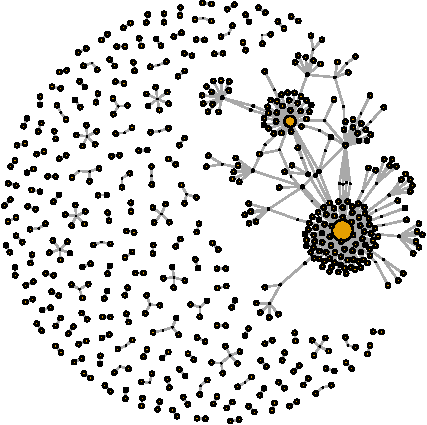
\includegraphics[keepaspectratio]{DataScience_files/figure-latex/unnamed-chunk-12-3.pdf}}

\begin{Shaded}
\begin{Highlighting}[]
\CommentTok{\# Extract relevant columns for competition analysis}
\NormalTok{edges\_competition }\OtherTok{\textless{}{-}}\NormalTok{ data }\SpecialCharTok{\%\textgreater{}\%} 
  \FunctionTok{select}\NormalTok{(}\AttributeTok{Company\_Name =} \StringTok{\textasciigrave{}}\AttributeTok{Company Name}\StringTok{\textasciigrave{}}\NormalTok{, }\AttributeTok{Competitor =} \StringTok{\textasciigrave{}}\AttributeTok{Competitors}\StringTok{\textasciigrave{}}\NormalTok{) }\SpecialCharTok{\%\textgreater{}\%}
  \FunctionTok{distinct}\NormalTok{()}

\CommentTok{\# Create an igraph object for competition analysis}
\NormalTok{network\_competition }\OtherTok{\textless{}{-}} \FunctionTok{graph\_from\_data\_frame}\NormalTok{(edges\_competition, }\AttributeTok{directed =} \ConstantTok{TRUE}\NormalTok{)}

\CommentTok{\# Plot the competition network}
\FunctionTok{plot}\NormalTok{(network\_competition, }\AttributeTok{vertex.label =} \ConstantTok{NA}\NormalTok{, }\AttributeTok{vertex.size =} \DecValTok{5}\NormalTok{, }\AttributeTok{edge.arrow.size =} \FloatTok{0.5}\NormalTok{)}
\end{Highlighting}
\end{Shaded}

\pandocbounded{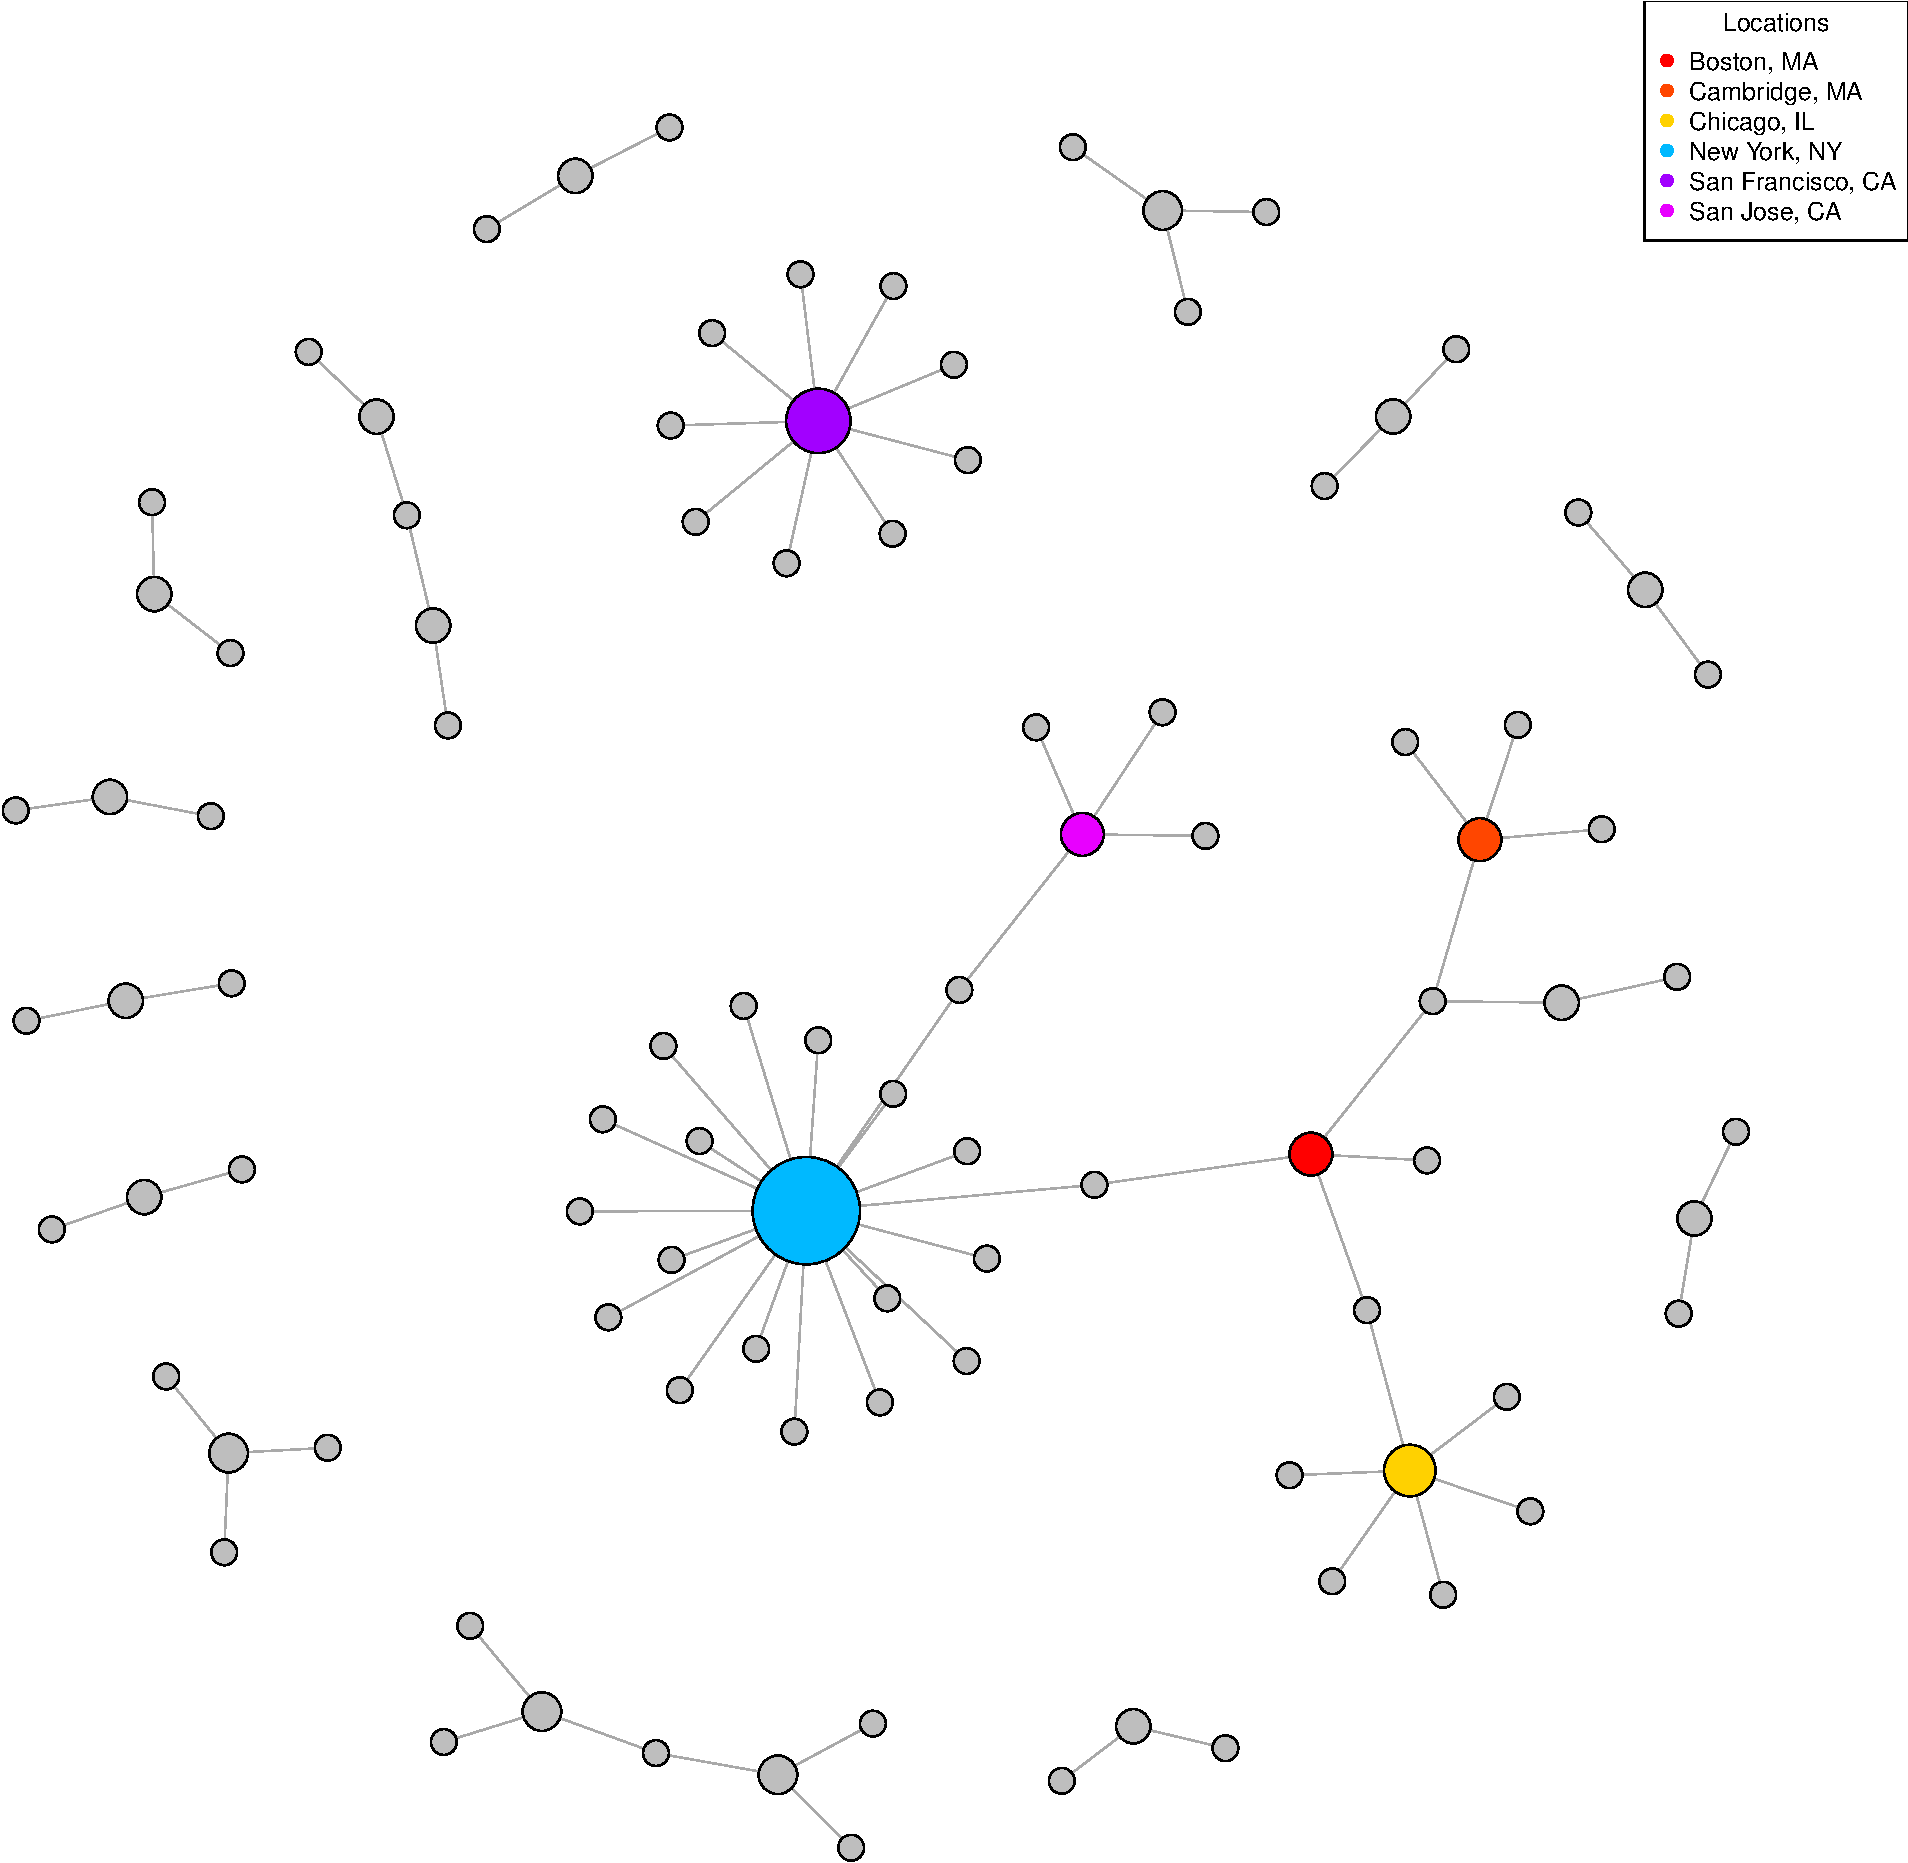
\includegraphics[keepaspectratio]{DataScience_files/figure-latex/unnamed-chunk-13-1.pdf}}

\subsection{Zweite Copilot iteration}\label{zweite-copilot-iteration}

\begin{Shaded}
\begin{Highlighting}[]
\CommentTok{\# Extrahiere Unternehmen und ihre Wettbewerber}
\NormalTok{edges }\OtherTok{\textless{}{-}}\NormalTok{ data }\SpecialCharTok{\%\textgreater{}\%}
  \FunctionTok{filter}\NormalTok{(}\SpecialCharTok{!}\FunctionTok{is.na}\NormalTok{(Competitors) }\SpecialCharTok{\&}\NormalTok{ Competitors }\SpecialCharTok{!=} \StringTok{"{-}1"}\NormalTok{) }\SpecialCharTok{\%\textgreater{}\%}
  \FunctionTok{separate\_rows}\NormalTok{(Competitors, }\AttributeTok{sep =} \StringTok{", "}\NormalTok{) }\SpecialCharTok{\%\textgreater{}\%}
  \FunctionTok{select}\NormalTok{(}\StringTok{\textasciigrave{}}\AttributeTok{Company Name}\StringTok{\textasciigrave{}}\NormalTok{, Competitors) }\SpecialCharTok{\%\textgreater{}\%}
  \FunctionTok{rename}\NormalTok{(}\AttributeTok{from =} \StringTok{\textasciigrave{}}\AttributeTok{Company Name}\StringTok{\textasciigrave{}}\NormalTok{, }\AttributeTok{to =}\NormalTok{ Competitors)}

\CommentTok{\# Erstelle den Graphen}
\NormalTok{g\_competitors }\OtherTok{\textless{}{-}} \FunctionTok{graph\_from\_data\_frame}\NormalTok{(edges, }\AttributeTok{directed =} \ConstantTok{FALSE}\NormalTok{)}

\CommentTok{\# Visualisiere das Netzwerk mit kleineren Knoten}
\FunctionTok{plot}\NormalTok{(g\_competitors, }\AttributeTok{vertex.label =} \ConstantTok{NA}\NormalTok{,}
     \AttributeTok{vertex.size =} \DecValTok{3}\NormalTok{,  }\CommentTok{\# Kleinere Knoten}
     \AttributeTok{edge.arrow.size =} \FloatTok{0.5}\NormalTok{,  }\CommentTok{\# Kleinere Pfeile}
     \AttributeTok{main =} \StringTok{"Unternehmensnetzwerk basierend auf Wettbewerbern"}\NormalTok{,}
\NormalTok{    )  }\CommentTok{\# Höhe der Grafik in Pixeln}
\end{Highlighting}
\end{Shaded}

\pandocbounded{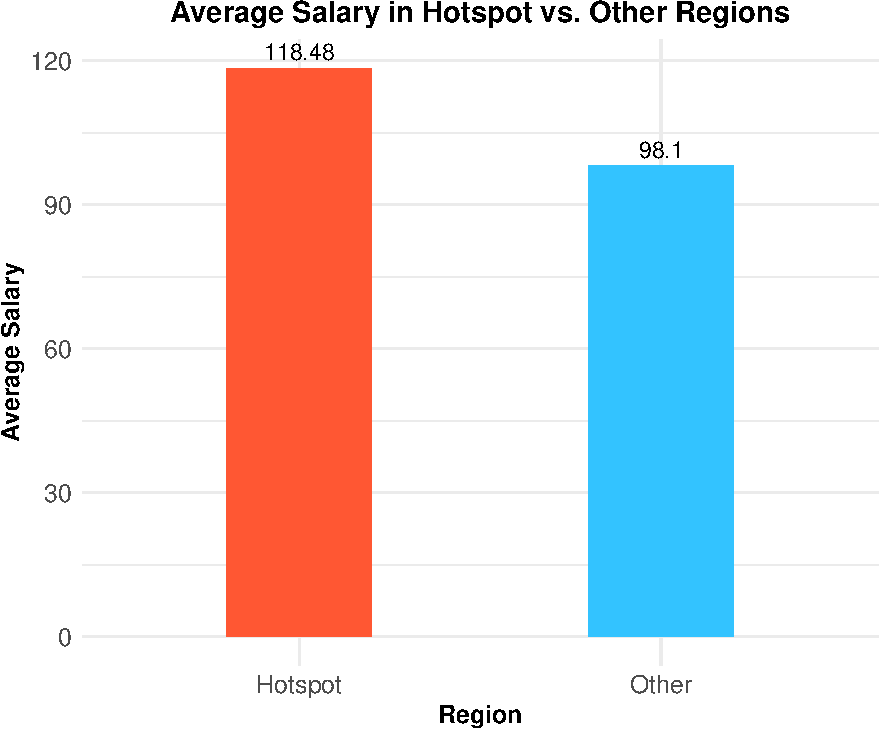
\includegraphics[keepaspectratio]{DataScience_files/figure-latex/unnamed-chunk-14-1.pdf}}

\begin{Shaded}
\begin{Highlighting}[]
\CommentTok{\# Calculate network metrics}
\NormalTok{degree\_centrality }\OtherTok{\textless{}{-}} \FunctionTok{degree}\NormalTok{(g\_competitors)}
\NormalTok{betweenness\_centrality }\OtherTok{\textless{}{-}} \FunctionTok{betweenness}\NormalTok{(g\_competitors)}
\NormalTok{closeness\_centrality }\OtherTok{\textless{}{-}} \FunctionTok{closeness}\NormalTok{(g\_competitors)}
\NormalTok{eigenvector\_centrality }\OtherTok{\textless{}{-}} \FunctionTok{eigen\_centrality}\NormalTok{(g\_competitors)}\SpecialCharTok{$}\NormalTok{vector}
\NormalTok{clustering\_coeff }\OtherTok{\textless{}{-}} \FunctionTok{transitivity}\NormalTok{(g\_competitors, }\AttributeTok{type =} \StringTok{"local"}\NormalTok{)}

\CommentTok{\# Detect communities}
\NormalTok{communities }\OtherTok{\textless{}{-}} \FunctionTok{cluster\_louvain}\NormalTok{(g\_competitors)}

\CommentTok{\# Prepare data for visNetwork}
\NormalTok{nodes }\OtherTok{\textless{}{-}} \FunctionTok{data.frame}\NormalTok{(}\AttributeTok{id =} \FunctionTok{V}\NormalTok{(g\_competitors)}\SpecialCharTok{$}\NormalTok{name,}
                    \AttributeTok{label =} \FunctionTok{V}\NormalTok{(g\_competitors)}\SpecialCharTok{$}\NormalTok{name,}
                    \AttributeTok{group =} \FunctionTok{membership}\NormalTok{(communities),}
                    \AttributeTok{value =}\NormalTok{ degree\_centrality,}
                    \AttributeTok{title =} \FunctionTok{paste}\NormalTok{(}\StringTok{"Degree:"}\NormalTok{, degree\_centrality, }\StringTok{"\textless{}br\textgreater{}Betweenness:"}\NormalTok{, betweenness\_centrality, }\StringTok{"\textless{}br\textgreater{}Closeness:"}\NormalTok{, closeness\_centrality, }\StringTok{"\textless{}br\textgreater{}Eigenvector:"}\NormalTok{, eigenvector\_centrality))}

\NormalTok{edges }\OtherTok{\textless{}{-}} \FunctionTok{data.frame}\NormalTok{(}\AttributeTok{from =} \FunctionTok{as.character}\NormalTok{(edges}\SpecialCharTok{$}\NormalTok{from), }\AttributeTok{to =} \FunctionTok{as.character}\NormalTok{(edges}\SpecialCharTok{$}\NormalTok{to))}

\CommentTok{\# Create interactive network visualization}
\FunctionTok{visNetwork}\NormalTok{(nodes, edges) }\SpecialCharTok{\%\textgreater{}\%}
  \FunctionTok{visOptions}\NormalTok{(}\AttributeTok{highlightNearest =} \ConstantTok{TRUE}\NormalTok{, }\AttributeTok{nodesIdSelection =} \ConstantTok{TRUE}\NormalTok{) }\SpecialCharTok{\%\textgreater{}\%}
  \FunctionTok{visGroups}\NormalTok{(}\AttributeTok{groupname =} \StringTok{"1"}\NormalTok{, }\AttributeTok{color =} \StringTok{"red"}\NormalTok{) }\SpecialCharTok{\%\textgreater{}\%}
  \FunctionTok{visGroups}\NormalTok{(}\AttributeTok{groupname =} \StringTok{"2"}\NormalTok{, }\AttributeTok{color =} \StringTok{"blue"}\NormalTok{) }\SpecialCharTok{\%\textgreater{}\%}
  \FunctionTok{visGroups}\NormalTok{(}\AttributeTok{groupname =} \StringTok{"3"}\NormalTok{, }\AttributeTok{color =} \StringTok{"green"}\NormalTok{) }\SpecialCharTok{\%\textgreater{}\%}
  \FunctionTok{visLayout}\NormalTok{(}\AttributeTok{randomSeed =} \DecValTok{123}\NormalTok{) }\SpecialCharTok{\%\textgreater{}\%}
  \FunctionTok{visLegend}\NormalTok{()}
\end{Highlighting}
\end{Shaded}

\begin{Shaded}
\begin{Highlighting}[]
\CommentTok{\# Print top nodes for each centrality measure}
\FunctionTok{print}\NormalTok{(}\StringTok{"Top 5 nodes by degree centrality:"}\NormalTok{)}
\end{Highlighting}
\end{Shaded}

\begin{verbatim}
## [1] "Top 5 nodes by degree centrality:"
\end{verbatim}

\begin{Shaded}
\begin{Highlighting}[]
\FunctionTok{print}\NormalTok{(}\FunctionTok{head}\NormalTok{(}\FunctionTok{sort}\NormalTok{(degree\_centrality, }\AttributeTok{decreasing =} \ConstantTok{TRUE}\NormalTok{), }\DecValTok{5}\NormalTok{))}
\end{Highlighting}
\end{Shaded}

\begin{verbatim}
##   Takeda Pharmaceuticals              AstraZeneca Liberty Mutual Insurance 
##                       42                       33                       31 
##                     PNNL                 Novartis 
##                       30                       25
\end{verbatim}

\begin{Shaded}
\begin{Highlighting}[]
\FunctionTok{print}\NormalTok{(}\StringTok{"Top 5 nodes by betweenness centrality:"}\NormalTok{)}
\end{Highlighting}
\end{Shaded}

\begin{verbatim}
## [1] "Top 5 nodes by betweenness centrality:"
\end{verbatim}

\begin{Shaded}
\begin{Highlighting}[]
\FunctionTok{print}\NormalTok{(}\FunctionTok{head}\NormalTok{(}\FunctionTok{sort}\NormalTok{(betweenness\_centrality, }\AttributeTok{decreasing =} \ConstantTok{TRUE}\NormalTok{), }\DecValTok{5}\NormalTok{))}
\end{Highlighting}
\end{Shaded}

\begin{verbatim}
##                     Booz Allen Hamilton                                  Gallup 
##                                841.8485                                749.0000 
##                           PA Consulting                      McKinsey & Company 
##                                715.4191                                713.0000 
## General Dynamics Information Technology 
##                                695.0000
\end{verbatim}

\begin{Shaded}
\begin{Highlighting}[]
\FunctionTok{print}\NormalTok{(}\StringTok{"Top 5 nodes by closeness centrality:"}\NormalTok{)}
\end{Highlighting}
\end{Shaded}

\begin{verbatim}
## [1] "Top 5 nodes by closeness centrality:"
\end{verbatim}

\begin{Shaded}
\begin{Highlighting}[]
\FunctionTok{print}\NormalTok{(}\FunctionTok{head}\NormalTok{(}\FunctionTok{sort}\NormalTok{(closeness\_centrality, }\AttributeTok{decreasing =} \ConstantTok{TRUE}\NormalTok{), }\DecValTok{5}\NormalTok{))}
\end{Highlighting}
\end{Shaded}

\begin{verbatim}
##               Esri             CareDx Medidata Solutions            Factual 
##                  1                  1                  1                  1 
##       Pitney Bowes 
##                  1
\end{verbatim}

\begin{Shaded}
\begin{Highlighting}[]
\FunctionTok{print}\NormalTok{(}\StringTok{"Top 5 nodes by eigenvector centrality:"}\NormalTok{)}
\end{Highlighting}
\end{Shaded}

\begin{verbatim}
## [1] "Top 5 nodes by eigenvector centrality:"
\end{verbatim}

\begin{Shaded}
\begin{Highlighting}[]
\FunctionTok{print}\NormalTok{(}\FunctionTok{head}\NormalTok{(}\FunctionTok{sort}\NormalTok{(eigenvector\_centrality, }\AttributeTok{decreasing =} \ConstantTok{TRUE}\NormalTok{), }\DecValTok{5}\NormalTok{))}
\end{Highlighting}
\end{Shaded}

\begin{verbatim}
## Takeda Pharmaceuticals               Novartis                 Pfizer 
##              1.0000000              0.6885416              0.5750772 
##                 Baxter            AstraZeneca 
##              0.5510613              0.3694600
\end{verbatim}

\begin{Shaded}
\begin{Highlighting}[]
\FunctionTok{print}\NormalTok{(}\StringTok{"Top 5 nodes by clustering coefficient:"}\NormalTok{)}
\end{Highlighting}
\end{Shaded}

\begin{verbatim}
## [1] "Top 5 nodes by clustering coefficient:"
\end{verbatim}

\begin{Shaded}
\begin{Highlighting}[]
\FunctionTok{print}\NormalTok{(}\FunctionTok{head}\NormalTok{(}\FunctionTok{sort}\NormalTok{(clustering\_coeff, }\AttributeTok{decreasing =} \ConstantTok{TRUE}\NormalTok{), }\DecValTok{5}\NormalTok{))}
\end{Highlighting}
\end{Shaded}

\begin{verbatim}
## CNH Industrial        Vermeer   L&T Infotech    Caterpillar        Pactera 
##      1.0000000      0.6666667      0.6666667      0.3333333      0.3333333
\end{verbatim}

\begin{Shaded}
\begin{Highlighting}[]
\CommentTok{\# Standort{-}Cluster für Gehälter und Bewertungen}
\NormalTok{edges\_location\_salary }\OtherTok{\textless{}{-}}\NormalTok{ data }\SpecialCharTok{\%\textgreater{}\%}
  \FunctionTok{select}\NormalTok{(Location, }\StringTok{\textasciigrave{}}\AttributeTok{Salary Estimate}\StringTok{\textasciigrave{}}\NormalTok{) }\SpecialCharTok{\%\textgreater{}\%}
  \FunctionTok{distinct}\NormalTok{() }\SpecialCharTok{\%\textgreater{}\%}
  \FunctionTok{mutate}\NormalTok{(}\StringTok{\textasciigrave{}}\AttributeTok{Salary Estimate}\StringTok{\textasciigrave{}} \OtherTok{=} \FunctionTok{as.numeric}\NormalTok{(}\FunctionTok{gsub}\NormalTok{(}\StringTok{"[\^{}0{-}9]"}\NormalTok{, }\StringTok{""}\NormalTok{, }\StringTok{\textasciigrave{}}\AttributeTok{Salary Estimate}\StringTok{\textasciigrave{}}\NormalTok{))) }\SpecialCharTok{\%\textgreater{}\%}
  \FunctionTok{drop\_na}\NormalTok{() }\SpecialCharTok{\%\textgreater{}\%}
  \FunctionTok{rename}\NormalTok{(}\AttributeTok{from =}\NormalTok{ Location, }\AttributeTok{to =} \StringTok{\textasciigrave{}}\AttributeTok{Salary Estimate}\StringTok{\textasciigrave{}}\NormalTok{)}

\CommentTok{\# Remove duplicate edges}
\NormalTok{edges\_location\_salary }\OtherTok{\textless{}{-}}\NormalTok{ edges\_location\_salary }\SpecialCharTok{\%\textgreater{}\%}
  \FunctionTok{distinct}\NormalTok{(from, to, }\AttributeTok{.keep\_all =} \ConstantTok{TRUE}\NormalTok{)}

\CommentTok{\# Erstelle den Graphen}
\NormalTok{g\_location\_salary }\OtherTok{\textless{}{-}} \FunctionTok{graph\_from\_data\_frame}\NormalTok{(edges\_location\_salary, }\AttributeTok{directed =} \ConstantTok{FALSE}\NormalTok{)}

\CommentTok{\# Visualisiere das Netzwerk}
\FunctionTok{plot}\NormalTok{(g\_location\_salary, }\AttributeTok{vertex.label =} \ConstantTok{NA}\NormalTok{, }\AttributeTok{vertex.size =} \DecValTok{5}\NormalTok{, }
     \AttributeTok{edge.arrow.size =} \FloatTok{0.5}\NormalTok{, }\AttributeTok{main =} \StringTok{"Standort{-}Cluster für Gehälter und Bewertungen"}\NormalTok{)}
\end{Highlighting}
\end{Shaded}

\pandocbounded{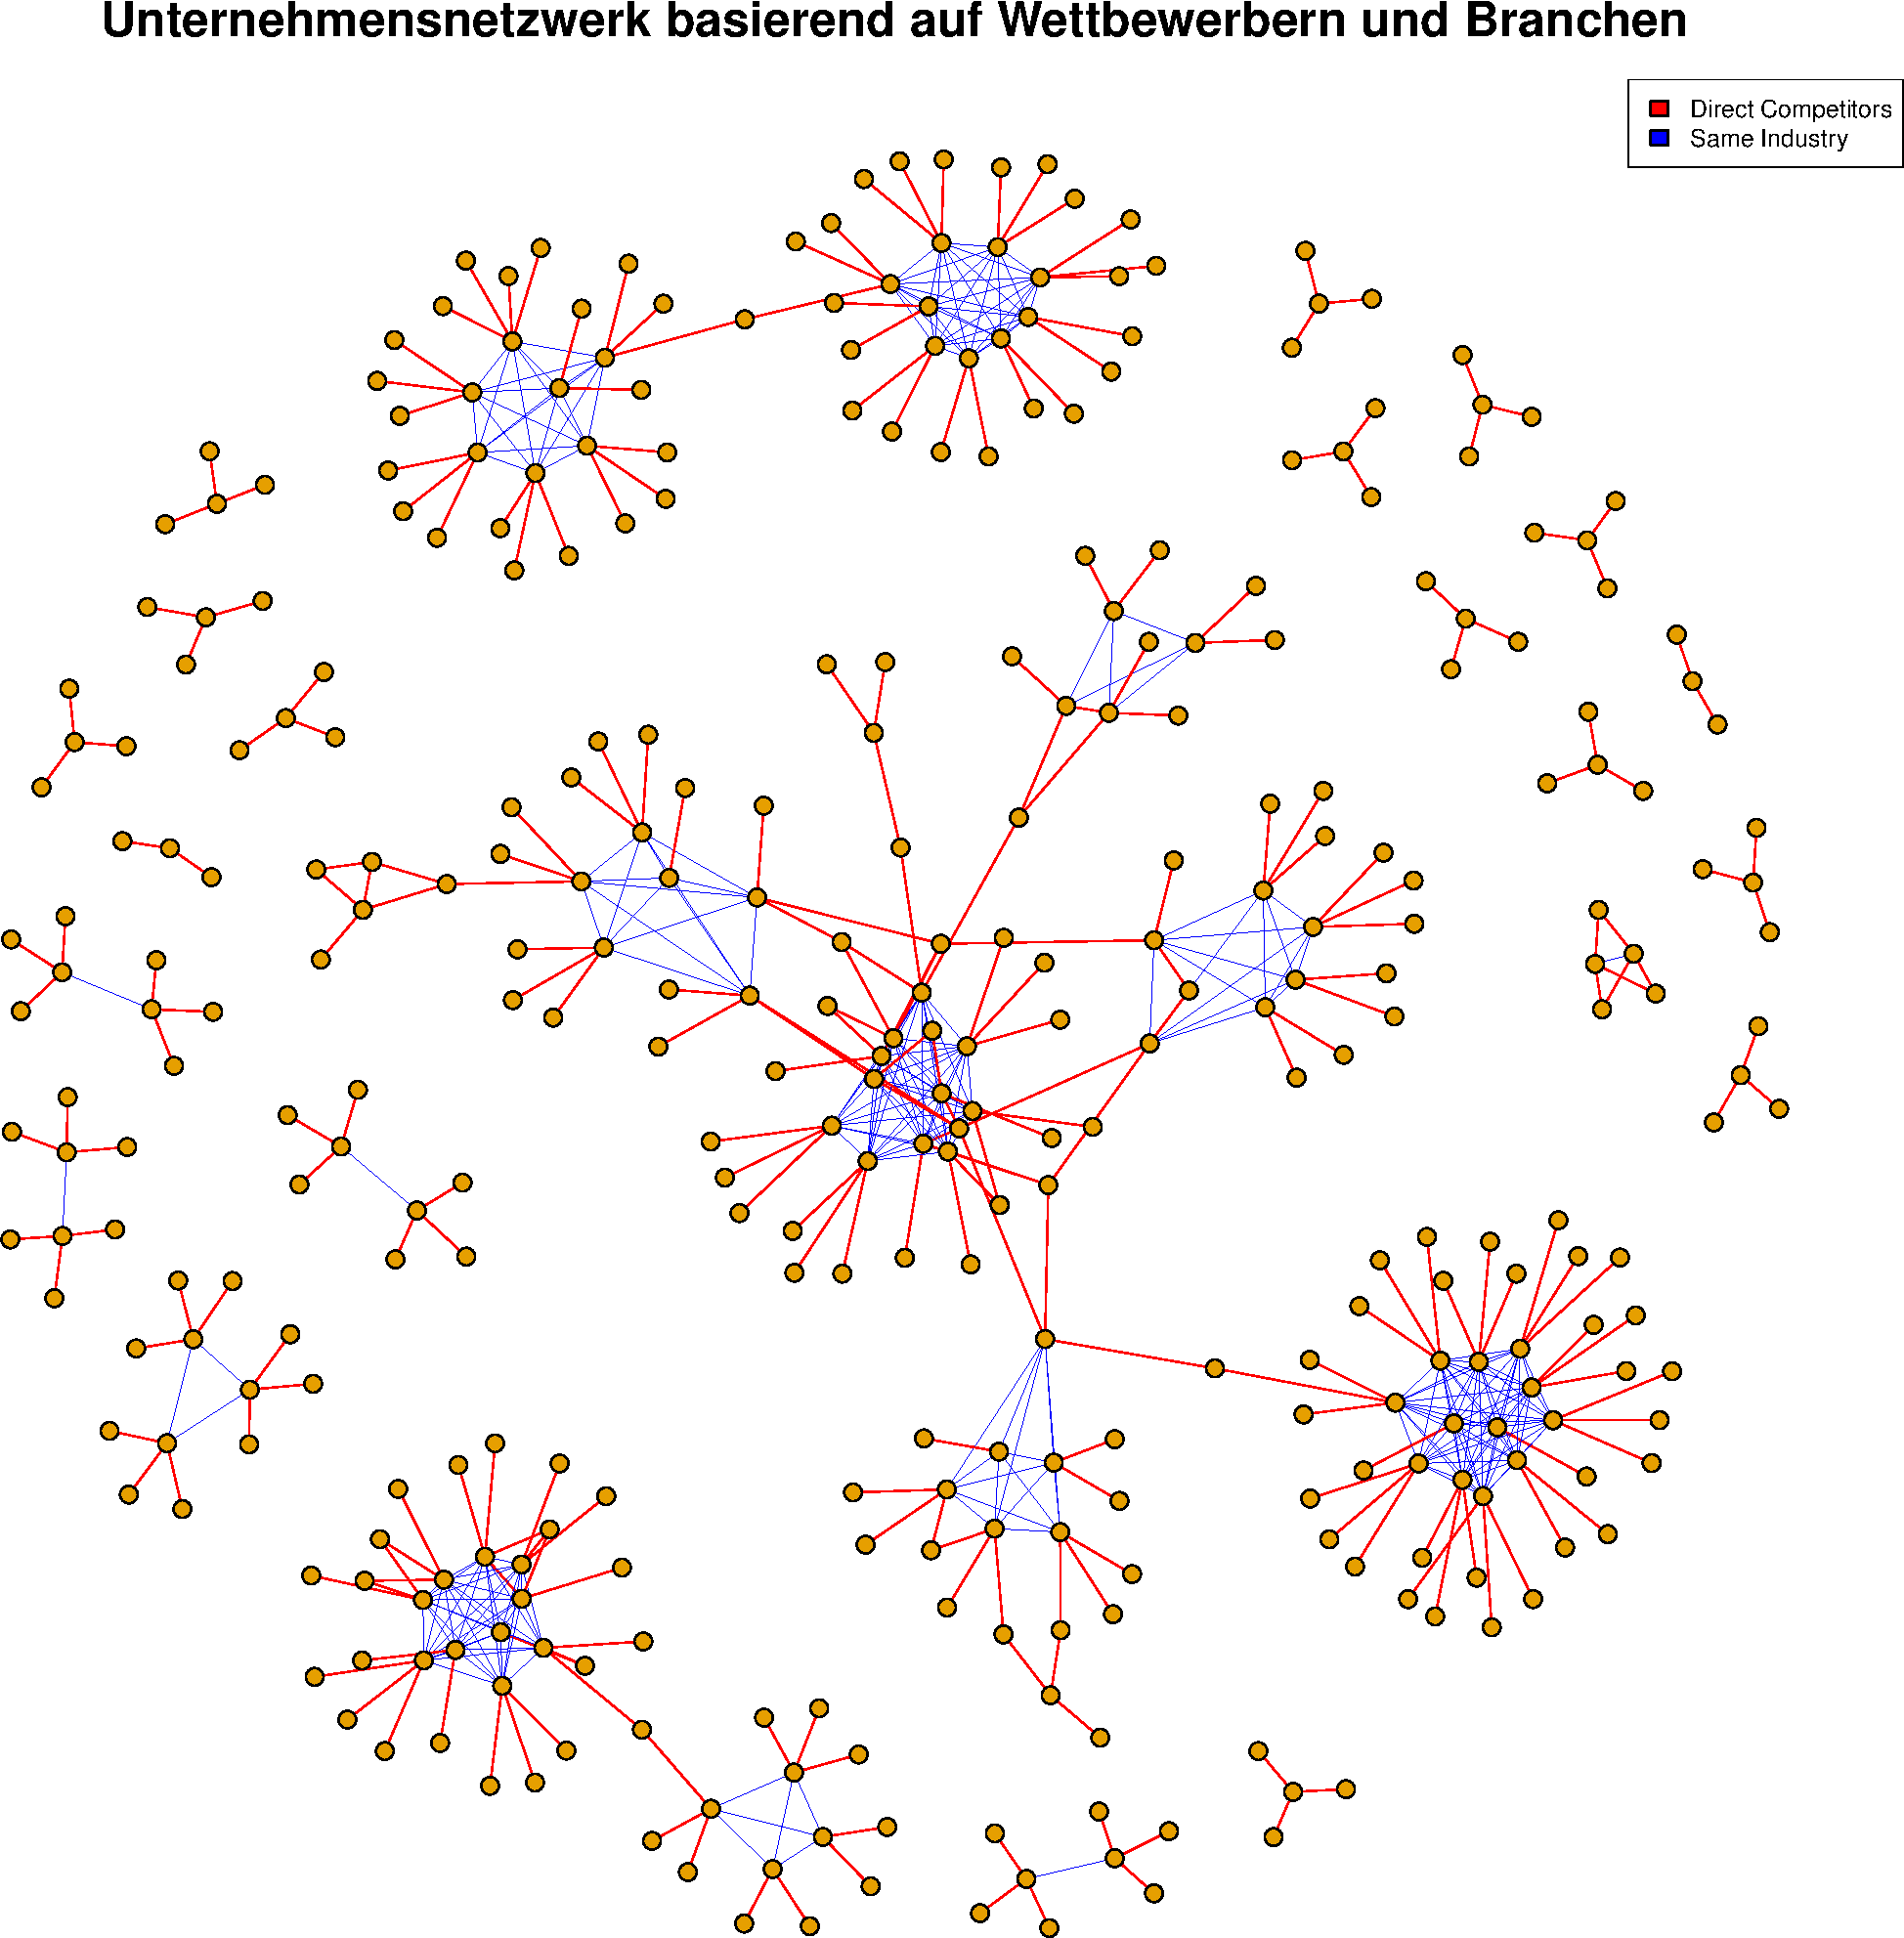
\includegraphics[keepaspectratio]{DataScience_files/figure-latex/unnamed-chunk-15-1.pdf}}

\section{Conclusion}\label{conclusion}

\ldots..

\section{Literaturverzeichnis}\label{literaturverzeichnis}

Davenport, Thomas H.; Patil, D. J. 2012. »Data Scientist: The Sexiest
Job of the 21st Century«, in Harvard Business Review vom 1. Oktober
2012.
\url{https://hbr.org/2012/10/data-scientist-the-sexiest-job-of-the-21st-century}
(Zugriff vom 30.10.2024).

Google Trends,
\url{https://trends.google.com/trends/explore?date=all&q=\%22data\%20science\%22,\%22data\%20scientist\%22}
(Zugriff vom 30.10.2024).

\end{document}
